\chapterimage{09_Snov.jpg} % Chapter heading image

\chapter{Interakcija svetlobe s snovjo}
V tem poglavju bomo podrobneje obravnavali interakcijo svetlobe s snovjo, ki jo 
v najpreprostejši obliki opišemo z lomnim količnikom. Na poenostavljenem modelu
bomo spoznali odvisnost lomnega količnika od frekvence vpadnega valovanja in pojasnili
posledice disperzije. Zapisali bomo tudi lomni količnik za prevodne snovi ter
opisali dva zanimiva pojava: optično aktivnost in Faradayev pojav.

\section{Fazna in grupna hitrost}
V tretjem poglavju smo zapisali osnovno rešitev valovne enačbe
v neomejenem prostoru (enačba~\ref{eq:valovnaE}) v obliki ravnih valov 
(enačba~\ref{eq:ravnival}). Izračunali smo fazno hitrost,
to je hitrost premikanja ploskev konstantne faze in
jo zapisali kot razmerje krožne frekvence vpadne svetlobe 
in valovnega števila (enačba~\ref{eq:03_10}):
\boxeq{eq:09_25a}{
v_f = \frac{\omega}{k}
}
Fazno hitrost svetlobe navadno označimo s $c$ in jo zapišemo kot (enačba~\ref{eq:c}):
\beq
c = \frac{c_0}{n}.
\label{eq:09_01}
\eeq
Pri tem lomni količnik $n$ označuje razmerje med hitrostjo svetlobe v 
vakuumu $c_0$ in hitrostjo svetlobe v snovi $c$. Na splošno je lomni količnik odvisen 
od snovi, po kateri se svetloba širi, in tudi od frekvence vpadne svetlobe.

Obravnavajmo dve ravni valovanji z enakima amplitudama $E_0$, ki potujeta v isti smeri vzdolž
osi~$z$. Njuni frekvenci naj se le malo razlikujeta, zato ju zapišimo kot: 
$\omega_1=\omega + \Delta \omega$ in $\omega_2=\omega - \Delta \omega$, pripadajoči
valovni števili naj bosta: $k_1 = k + \Delta k $ in $k_2 = k - \Delta k$. 
Vsoto teh dveh valovanj zapišemo kot:
\begin{align}
E &= E_0 \cos (k_1z-\omega_1 t)+ E_0 \cos (k_2z-\omega_2 t) \nonumber\\
&= E_0 \cos\left((k+\Delta k)z-(\omega + \Delta \omega)t\right) 
+ E_0 \cos\left((k-\Delta k)z-(\omega - \Delta \omega)t\right)\nonumber \\
&= E_0 \cos\left((kz - \omega t) +(\Delta k z-\Delta \omega t\right)
+ E_0 \cos\left((k z - \omega t) - (\Delta k z- \Delta \omega t)  \right)\!. 
\label{eq:09_23}
\end{align}
Z uporabo adicijskega izreka za kotne funkcije:
\beq
\cos\alpha + \cos \beta = 2 \cos \frac{\alpha + \beta}{2} \cos \frac{\alpha - \beta}{2}
\eeq
izraz preoblikujemo v:
\beq
E = 2E_0 \cos \left(kz - \omega t \right)\cos \left(\Delta kz - \Delta \omega t \right)\!.
\label{eq:09_24}
\eeq
Vsota teh dveh valovanj je torej potujoče valovanje v smeri $z$ s frekvenco, ki je 
enaka osrednji krožni frekvenci $\omega$, in valovnim številom, ki je enako 
osrednjemu valovnemu številu $k$. Valovanje je amplitudno modulirano 
s krožno frekvenco $\Delta \omega$ (slika~\ref{fig:09_utripanje}).
\begin{figure}[ht]
\centering
\def\svgwidth{140truemm} 
\input{slike/09_vsota.pdf_tex}
\caption{Dve valovanji z različnima frekvencama (modra in zelena, levo) se seštejeta
v amplitudno modulirano valovanje (rdeča, desno). Črna črta označuje ovojnico valovanja.}
\label{fig:09_utripanje}
\end{figure}

Pri valovanju, ki predstavlja zaporedje potujočih sunkov, lahko določimo dve
različni hitrosti. Prva je hitrost premikanja ploskev konstantne
faze oziroma premikanja vrhov hitre modulacije. To je fazna hitrost, ki
jo izračunamo iz znane enačbe~(\ref{eq:09_25a}). Druga pa je hitrost, s katero
se premikajo vrhovi počasne modulacije oziroma posamezni sunki. Izračunamo jo
iz enačbe~(\ref{eq:09_24}) in dobimo 
\beq
v_g=\frac{z}{t} = \frac{\Delta \omega}{\Delta k}.
\eeq
Hitrost premikanja sunkov imenujemo grupna hitrost in jo 
v limiti majhnih frekvenčnih razlik zapišemo kot:
\boxeq{eq:09_24a}{
v_g = \frac{d\omega}{d k}.
}

Izraz za grupno hitrost smo izpeljali na primeru valovanja, sestavljenega iz dveh
valovanj, vendar velja na splošno za potovanje sunkov svetlobe. Informacija,
ki jo prenašajo sunki svetlobe, po snovi torej potuje z grupno hitrostjo.
\vglue5truemm
\begin{figure}[ht]
\centering
\def\svgwidth{130truemm} 
\input{slike/09_disperzija2.pdf_tex}
\caption{Posnetki potujočega amplitudno moduliranega valovanja ob različnih časih.
Potovanje posameznega vala, ki se premika z fazno hitrostjo, označuje zelena pika. Potovanje
amplitudne modulacije označuje modra pika in ta se premika z grupno 
hitrostjo. Vidimo, da sta v narisanem primeru fazna in grupna hitrost različni.}
\label{fig:09_disperzija}
\end{figure}

Vstavimo zvezo med valovnim številom in krožno frekvenco $k=\omega n /c_0$ v izraz za 
grupno hitrost (enačba~\ref{eq:09_24a}) in dobimo:
\beq
v_g = \frac{d\omega}{dk } = \left(\frac{dk}{d\omega}\right)^{-1} = \left( \frac{d}{d\omega}\left( 
\frac{\omega n }{c_0}\right)\!\right)^{-1}\!\!.
\label{eq:09_25}
\eeq
Upoštevamo, da je lomni količnik na splošno odvisen od frekvence valovanja, in zapišemo:
\beq
v_g = \left(\frac{n}{c_0} + \frac{\omega}{c_0 }\frac{dn}{d\omega}\right)^{-1} = 
\frac{c_0}{n+\omega \frac{dn}{d\omega}}.
\label{eq:09_26}
\eeq
V zapisanem izrazu za grupno hitrost nastopa odvod lomnega količnika po krožni frekvenci vpadnega
valovanja. Če je lomni količnik neodvisen od frekvence, je odvod enak nič in 
takrat sta fazna in grupna hitrost enaki. Na splošno je odvod različen od nič in v naslednjem razdelku bomo
spoznali, da je za večino snovi odvod na celotnem spektralnem območju vidne svetlobe pozitiven.
Na splošno zato velja, da je za vidno svetlobo grupna hitrost manjša od fazne.

\section{Lomni količnik}
\label{chap:lomni}
Odvisnost lomnega količnika od frekvence vpadnega 
elektromagnetnega valovanja bomo izračunali na preprostem modelu. 
Omejimo se na nemagnetne snovi, za katere je $\mu = 1$, kar pomeni, da
za izračun frekvenčne odvisnosti lomnega količnika zadošča poznati 
$\varepsilon(\omega)$. 

Naj bo snov sestavljena iz $N$
enakih atomov ali molekul, ki so enakomerno porazdeljeni
po prostoru s prostornino $V$. Za opis posameznega atoma ali molekule uporabimo 
klasični model oscilatorja, ki ga imenujemo Lorentzev model 
po nizozemskem fiziku Hendriku Lorentzu (1853--1928). 

Zamislimo si, da atom ali molekulo sestavljata kroglica 
pozitivnega naboja, ki miruje v izhodišču pri $x=0$, in kroglica
(oblak) negativnega naboja na neki ravnovesni oddaljenosti. Med njima naj 
deluje privlačna sila, ki jo v klasičnem modelu opišemo z vzmetjo
s konstanto vzmeti $k$ (slika~\ref{fig:09_Lorentz}). 
Poleg elastične sile naj na negativno nabito kroglico med 
premikanjem deluje tudi sila dušenja, ki opisuje absorpcijo svetlobe
v snovi. V klasični sliki si lahko
zamislimo, da je ravnovesna razdalja med kroglicama enaka $x_r$, 
v bolj realističnem modelu, v katerem elektron opišemo kot oblak okoli jedra,
pa je ravnovesna razdalja enaka 0. Podobno velja tudi za molekule, ki 
nimajo dipolnega momenta. Ker je razlika le v konstanti, 
to na končni rezultat ne vpliva.
\begin{figure}[ht]
\centering
\def\svgwidth{60truemm} 
\input{slike/09_Lorentz.pdf_tex}
\caption{Preprost Lorentzev model atoma. Zaradi vpadnega 
elektromagnetnega valovanja elektron vzbujeno niha.
}
\label{fig:09_Lorentz}
\vglue-5truemm
\end{figure}

Naj na tak model atoma ali molekule vpada elektromagnetno valovanje. Ker je 
valovna dolžina svetlobe bistveno večja od atoma, lahko privzamemo, da
je električno polje po velikosti znotraj celotnega atoma homogeno in enako $E$.
Za negativno nabito kroglico (elektron) zapišemo Newtonov zakon, pri čemer 
upoštevamo silo vzmeti, silo 
dušenja in silo na naboj v električnem polju. Omejimo se na polarizacijo 
polja v smeri $x$ in zapišemo:
\beq
m \ddot{x} = -kx -\gamma m \dot{x} - e_0 E.
\label{eq:09_02}
\eeq
Pri tem so $m$ masa negativno nabite kroglice, $\gamma$ koeficient dušenja
in $E = E_0\,e^{-i\omega t}$.

\begin{remark}
Pri zapisu Lorentzevega modela smo privzeli, da je električno polje, 
ki ga čuti atom, enako vpadnemu električnemu polju. 
To velja, dokler je atom sam ali če snov sestavlja redek plin. Če je 
atom v snovi obdan z ostalimi atomi, 
čuti tudi njihov vpliv, zato bi bilo pravilneje upoštevati skupni vpliv, ki 
ga zapišemo s tako imenovanim lokalnim poljem. 
Kako izračunamo vpliv lokalnega polja, bomo spoznali v naslednjem razdelku. 
\end{remark}

Vpeljemo lastno krožno frekvenco $\omega_0 = k/m$ in 
enačbo prepišemo v:
\beq
\ddot{x} + \gamma \dot{x} + \omega_0^2 x  = - \frac{e_0}{m} E_0 e^{-i \omega t}.
\label{eq:09_04}
\eeq
Rešujemo jo z nastavkom:
\beq
x(t) = x_0 e^{-i\omega t},
\label{eq:09_05}
\eeq
pri čemer $x_0$ opisuje amplitudo nihanja, odvisno od $\omega$. Vstavimo nastavek 
(enačba~\ref{eq:09_05}) v enačbo~(\ref{eq:09_04}) in dobimo:
\beq
-\omega^2 x_0 - i \omega \gamma x_0 + \omega_0^2 x_0  = - \frac{e_0}{m} E_0.
\label{eq:09_06}
\eeq
Od tod izrazimo amplitudo nihanja v odvisnosti od frekvence vpadnega valovanja:
\beq
x_0 = \frac{-e_0/m}{\omega_0^2 - \omega^2 - i\gamma \omega}~E_0.
\label{eq:09_07}
\eeq
V zapisanem izrazu prepoznamo značilno resonančno odvisnost dušenega nihala. 

Vpadno električno polje izmakne negativno nabito kroglico iz ravnovesne 
lege, kar povzroči nastanek dipolnega momenta $\mathbf{p}$:
\beq
\mathbf{p} = -e_0\,x\,\mathbf{e}_x.
\label{eq:09_08}
\eeq
Prehod iz mikroskopskega opisa z dipolnim momentom posameznega atoma 
v makroskopski opis naredimo z upoštevanjem gostote atomov v snovi 
$\varrho = N/V$. Vpeljemo inducirano električno polarizacijo $\mathbf{P}$, ki 
je enaka celotnemu dipolnemu momentu na enoto volumna:
\beq
\mathbf{P} = \frac{\mathbf{p}N}{V} = \mathbf{p}\,\varrho. 
\label{eq:09_09}
\eeq
Z upoštevanjem enačb~(\ref{eq:09_07} in \ref{eq:09_08}) zapišemo 
električno polarizacijo v snovi kot:
\beq
\mathbf{P} = -e_0\,x\,\mathbf{e}_x\,\varrho = \frac{e_0^2\,\varrho/m}{\omega_0^2 
- \omega^2 - i\gamma \omega}\,\mathbf{e}_x\,E_0\,e^{-i\omega t}.
\label{eq:09_10}
\eeq
Spomnimo se, da lahko inducirano električno polarizacijo izrazimo z jakostjo
električnega polja v snovi:
\beq
\mathbf{P} = \varepsilon_0 (\epsilon-1) \mathbf{E}.
\label{eq:09_12}
\eeq
\vglue-5truemm
\begin{remark}
Enačba~(\ref{eq:09_12}) je linearni približek zveze med električno polarizacijo in 
jakostjo električnega polja. Pri velikih vpadnih jakostih električnega polja linearna zveza 
ne velja in treba je upoštevati tudi višje člene v razvoju z višjimi potencami polja. Ti
opisujejo nelinearne optične pojave, kar presega okvir te knjige.
\end{remark}

Enačbo~(\ref{eq:09_12}) primerjamo z enačbo~(\ref{eq:09_10}) in dobimo:
\beq
\varepsilon= 1 + \frac{e_0^2\,\varrho/\varepsilon_0 m}{\omega_0^2 - \omega^2 - i\gamma \omega}.
\label{eq:09_13}
\eeq
Vpeljemo še tako imenovano plazemsko frekvenco:
\beq
\omega_p = \sqrt{\frac{e_0^2\,\varrho }{\varepsilon_0 m}}
\label{eq:09_14}
\eeq
in upoštevamo zvezo med dielektričnostjo in na splošno kompleksnim lomnim količnikom:
\beq
\varepsilon = \mathcal{N}^2.
\label{eq:09_15}
\eeq
Dobimo:
\boxeq{eq:09_16}{
\varepsilon = \mathcal{N}^2 = 1+ \frac{\omega_p^2}{\omega_0^2 - \omega^2 - i\gamma \omega}.
}
\begin{remark}
V plazmi se elektroni prosto gibljejo in niso vezani na atome,
zato za njih velja $k=0$ in $\gamma = 0$. Za opis njihovega
gibanja ostane le še krožna frekvenca $\omega_p$, od tod ime plazemska frekvenca.
\end{remark}

Kompleksni lomni količnik $\mathcal{N}$ razdelimo na realni $n'$ in imaginarni del $n''$ in 
zapišemo:
\beq
\mathcal{N}^2 = (n'+in'')^2 = n'^2-n''^2+2in'n'' =  1+ \frac{\omega_p^2}{\omega_0^2 - \omega^2 - i\gamma \omega}.
\label{eq:09_17}
\eeq
Izenačimo realni in imaginarni del leve in desne strani enačbe. Dobimo:
\beq
n'^2 -n''^2 = \varepsilon' = 1 + \frac{\left(\omega_0^2 - \omega^2\right)\omega_p^2}{\left(\omega_0^2 - 
\omega^2\right)^2 + \gamma^2 \omega^2}
\label{eq:09_18}
\eeq
ter 
\beq
2n'n'' = \varepsilon'' = \frac{\gamma \omega \omega_p^2}{\left(\omega_0^2 - 
\omega^2\right)^2 + \gamma^2 \omega^2}.
\label{eq:09_19}
\eeq
Zapisali smo sistem dveh enačb za realni in imaginarni del lomnega količnika. Rešujemo ga podobno kot
sistem enačb za lomni količnik v prevodni snovi (enačbe~\ref{eq:nkompleks2} in \ref{eq:03_72})
z rešitvami v obliki enačb~(\ref{eq:03_76} in \ref{eq:03_77}). Rešitvi sta:
\beq
n'^2 = \frac{1}{2}\left(\varepsilon'+\sqrt{\varepsilon'^2 + \varepsilon''^2}\right)
\label{eq:09_20}
\eeq
in
\beq
n''^2 = \frac{1}{2}\left(-\varepsilon'+\sqrt{\varepsilon'^2 + \varepsilon''^2}\right)\!,
\label{eq:09_21}
\eeq
pri čemer sta $\varepsilon'$ in $\varepsilon''$ podana z enačbama~(\ref{eq:09_18} in \ref{eq:09_19}).
Realni in imaginarni del lomnega količnika sta tako odvisna od frekvence vpadnega valovanja. 
Odvisnost lomnega količnika od frekvence vpadnega elektromagnetnega valovanja, zaradi katere
se fazna in grupna hitrost valovanja v snovi razlikujeta, imenujemo disperzija.

\section{Disperzija}
Na preprostem modelu smo izpeljali lomni količnik snovi in pokazali,
kako se njegov realni in imaginarni del
spreminjata s frekvenco vpadnega elektromagnetnega valovanja. Ker so izrazi
razmeroma zapleteni, se navadno poslužimo približkov. Prvi naj 
bo približek redkega plina. 

V redkem plinu vrednost lomnega količnika le malo odstopa od lomnega količnika vakuuma 
in $\mathcal{N} \approx 1$. Lomni količnik (enačba~\ref{eq:09_17}) zato lahko razvijemo in dobimo:
\begin{align}
\mathcal{N} &= \sqrt{1+ \frac{\omega_p^2}{\omega_0^2 - \omega^2 - i\gamma \omega}} \\
&\approx 1 + \frac{1}{2}\frac{\left(\omega_0^2 - \omega^2\right)\omega_p^2}{\left(\omega_0^2 - 
\omega^2\right)^2 + \gamma^2 \omega^2} + \frac{i}{2}\frac{\gamma \omega \omega_p^2}{\left(\omega_0^2 - 
\omega^2\right)^2 + \gamma^2 \omega^2}.
\label{eq:09_22}
\end{align}
\begin{figure}[h!]
\centering
\def\svgwidth{140truemm} 
\input{slike/09_real_im_n.pdf_tex}
\caption{Odvisnost realnega (a) in imaginarnega dela (b) lomnega količnika od 
frekvence vpadne svetlobe v preprostem Lorentzevem modelu redkega plina. Osenčeni del na levi 
sliki označuje območje anomalne disperzije.}
\label{fig:09_nkompleks}
\end{figure}

Poglejmo najprej realni del lomnega količnika (slika~\ref{fig:09_nkompleks}\,a). 
Pri majhnih vrednostih je lomni količnik nekoliko večji od 1, 
njegova velikost pa je odvisna od razmerja med plazemsko in lastno frekvenco.
V bližini lastne frekvence $\omega_0$ lomni količnik naraste, nato strmo pade, potem pa 
začne ponovno naraščati in se počasi približuje vrednosti 1. V skoraj celotnem 
spektralnem območju je tako odvod lomnega količnika po frekvenci pozitiven 
(območje normalne disperzije), razen v ozkem območju v bližini lastne 
frekvence $\omega_0$, kjer je odvod negativen (območje anomalne disperzije). 
Za zelo velike frekvence vpadne svetlobe je lomni količnik približno enak 1.

Izkaže se, da za večino snovi lastna frekvenca $\omega_0$
leži v ultravijoličnem delu spektra, torej pri frekvencah, ki so večje od
frekvenc vidne svetlobe. Posledično je lomni količnik za vidno svetlobo 
vedno večji od 1. Za zelo velike frekvence, na primer za rentgensko svetlobo,
je lomni količnik manjši od 1. Lomni količnik kremena pri valovni 
dolžini $0,5~\si{nm}$ je tako $0,9998$. 
\begin{figure}[h]
\centering
\def\svgwidth{80truemm} 
\input{slike/09_stekla1.pdf_tex}
\caption{Odvisnosti lomnega količnika od valovne dolžine za nekaj različnih vrst stekel. SF10
 in F2 sta kremenovi stekli, BK7 pa je borosilikatno kronsko steklo. Osenčeni 
 del označuje vidni del spektra.}
\label{fig:09_stekla}
\end{figure}

Odvod lomnega količnika po frekvenci vpadne svetlobe $dn/d\omega$
je za vse frekvence, razen v bližini $\omega_0$, pozitiven. 
Ker so frekvence vidne svetlobe manjše od lastnih frekvenc, je celotna
vidna svetloba v območju normalne disperzije, kar pomeni, da z naraščajočo
frekvenco lomni količnik narašča in z naraščajočo valovno dolžino pojema (slika~\ref{fig:09_stekla}). 
Po enačbi~(\ref{eq:09_26}) to pomeni, da je grupna hitrost vpadne vidne 
svetlobe vedno manjša od fazne hitrosti. 

Poglejmo še imaginarni del lomnega količnika (slika~\ref{fig:09_nkompleks}\,b), ki 
opisuje absorpcijo svetlobe. Večinoma je enak nič, razen v bližini lastne frekvence. 
V območju anomalne disperzije, v katerem je grupna hitrost večja od fazne, se 
torej vpadna svetloba močno absorbira. 

\begin{remark}
Vpadna svetloba se lahko absorbira zaradi različnih pojavov. To so lahko 
elektronski prehodi (tipično v vidnem ali ultravijoličnem delu spektra), 
vzbujanje vibracijskih stanj v snovi (infrardeč del spektra) ali 
vzbujanje rotacijskih stanj (v mikrovalovnem delu spektra).
\end{remark}

Disperzijo smo pojasnili na preprostem Lorentzevem modelu.
V dejanski snovi oziroma atomskem/molekulskem sistemu je navadno več resonanc, pri čemer
vsaki od njih ustrezata neka resonančna frekvenca $\omega_{0j}$ in koeficient
dušenja $\gamma_j$. Potem vse prispevke zapišemo kot vsoto posameznih prispevkov 
z ustreznimi amplitudami $f_j$:
\beq
\varepsilon = \mathcal{N}^2 = 1+ \sum_j \frac{f_j \omega_{pj}^2}{\omega_{0j}^2 - \omega^2 - i\gamma_j\omega}.
\label{eq:09_27}
\eeq
\begin{figure}[h!]
\centering
\def\svgwidth{140truemm} 
\input{slike/09_disp_multi.pdf_tex}
\caption{Primer disperzije realnega dela lomnega količnika za Lorentzev model 
z več lastnimi resonancami. Senčeni del označuje območje vidne svetlobe, 
za katero velja normalna disperzija.}
\label{fig:09_disp_multi}
\end{figure}

V praksi za enačbo~(\ref{eq:09_27}) uporabimo različne približke, ki v danem frekvenčnem
območju dovolj dobro opišejo odvisnost lomnega količnika. V prozornih snoveh lahko 
dušenje, ki na splošno povzroča absorpcijo, zanemarimo in privzamemo $\gamma_j = 0$ za 
vsak $j$. V tem približku dobimo:
\beq
\mathcal{N}^2 = n'^2 = 1+ \sum_j \frac{f_j \omega_{pj}^2}{\omega_{0j}^2 - \omega^2}.
\label{eq:09_28}
\eeq
Namesto krožne frekvence lahko vstavimo tudi valovno dolžino svetlobe in dobimo:
\beq
n'^2 = 1 + \sum_j \frac{f_j \omega_{pj}^2\lambda_{oj}^2\lambda^2}{\lambda^2 - \lambda_{0j}^2}.
\label{eq:09_29}
\eeq
Kadar je valovna dolžina vpadne svetlobe razmeroma blizu ene lastne frekvence (a še vedno 
dovolj daleč, da je v območju normalne disperzije), je navadno tako daleč
od ostalih, da lahko prispevke ostalih lastnih frekvenc upoštevamo le v konstanti. Ostane:
\boxeq{eq:09_30}{
n'^2 = A + \sum_j \frac{G_j \lambda^2}{\lambda^2 - \lambda_{0j}^2}.
}
Približek je leta 1872 zapisal nemški fizik Wolfgang von Sellmeier, zato ga danes
imenujemo Sellmeierjeva enačba. Ta zveza se pogosto uporablja za opis disperzije 
lomnega količnika $n(\lambda)$ v prozornih snoveh. 

Še preprostejši je Cauchyjev približek, ki ga imenujemo po francoskem matematiku
Augustin-Louisu Cauchyju (1789--1857). Uporabimo ga lahko, kadar je izbrano spektralno
območje dovolj daleč od resonanc. Poleg tega upoštevamo, da se lomni količnik le malo 
razlikuje od 1, in zapišemo:
\boxeq{eq:09_30a}{
n = A + \frac{B}{\lambda^2}.
}
\vglue3truemm
\begin{example}{\bf Cauchyjev približek za lomni količnik.}
Najpreprostejši opis odvisnosti lomnega količnika od valovne dolžine vpadne svetlobe
je Cauchyjev približek. Čeprav smo zvezo izračunali za redke pline, velja v vidnem
območju dovolj dobro tudi
za gostejše trdne snovi. Nekaj parametrov $A$ in $B$ za izračun lomnega količnika
je podanih v tabeli:
\vglue2truemm
\begin{center}
\begin{tabular}{|l|l|l|}
\hline
snov& $A$ & $B~[\si{\micro\metre}^2]$\\ \hline 
taljeno kremenovo steklo & 1,4580 & 0,00354\\ \hline
kronsko steklo K5 & 1,5220 & 0,00459\\ \hline
svinčevo steklo SF10 & 1,7280 & 0,01342\\ \hline
\end{tabular}
\end{center}
\end{example}

\subsection*{Popravek lokalnega polja v gosti snovi}
Do zdaj smo obravnavali redko snov, v kateri so atomi oziroma molekule
dovolj oddaljeni, da ne čutijo medsebojnega vpliva. 
Zato smo v preprostem Lorentzevem modelu za polje, ki ga čuti elektron, 
vzeli kar polje vpadne svetlobe $E$. Če pa je izbrana molekula obdana
z drugimi molekulami, ki se pod vplivom zunanjega električnega polja 
polarizirajo, se  električno polje na mestu izbrane 
molekule spremeni. Za izračun tako imenovanega lokalnega polja $\tilde{E}$
moramo upoštevati tudi okoliško polarizacijo.

Lokalnega polja na tem mestu ne bomo izračunali (glej npr. Born in Wolf, {\it
Principles of Optics}), zapišimo le, da v izotropnih snoveh velja:
\beq
\tilde{E} = E + \frac{P}{3\varepsilon_0},
\label{eq:09_31}
\eeq
pri čemer smo se omejili le na eno smer, zato smo vektorski zapis opustili. 
Prvi člen v enačbi~(\ref{eq:09_31}) predstavlja jakost električnega 
polja vpadne svetlobe, drugi člen pa opisuje polarizacijsko 
polje zaradi okoliških molekul. 

Z uporabo zveze
$P = \varepsilon_0 (\varepsilon -1) E$ dobimo:
\beq
\tilde{E} = E + \frac{\varepsilon_0 (\varepsilon -1) E}{3\varepsilon_0} = 
\frac{\epsilon + 2}{3}E.
\label{eq:09_32}
\eeq
Jakost lokalnega polja je tako sorazmerna jakosti vpadnega polja, sorazmernostni
faktor pa je odvisen od dielektričnosti snovi.

Pri izračunu inducirane polarizacije v snovi (enačba~\ref{eq:09_10}) 
moramo zaradi vpliva sosednjih molekul upoštevati $\tilde{E}$. Sledi:
\beq
P = \frac{e_0^2\,\varrho/m}{\omega_0^2 - \omega^2 -i\gamma \omega}
\frac{\varepsilon+2}{3}\,E_0\,e^{-i\omega t}
= \varepsilon_0 (\varepsilon -1) E_0\,e^{-i\omega t}.
\label{eq:09_33}
\eeq
Od tod izračunamo zvezo:
\beq
\frac{\varepsilon -1 }{\varepsilon+2} = \frac{\mathcal{N}^2-1}{\mathcal{N}^2+2} = 
\frac{\omega_p^2/3}{\omega_0^2 - \omega^2 - i\gamma \omega}.
\label{eq:09_34}
\eeq
Če je krožna frekvenca vpadne svetlobe daleč od lastnih frekvenc, lahko dušenje zanemarimo in 
izraz preoblikujemo v:
\beq
\frac{\varepsilon -1 }{\varepsilon+2} = \frac{\mathcal{N}^2-1}{\mathcal{N}^2+2} = 
\frac{\omega_p^2}{3\left(\omega_0^2 - \omega^2\right)}.
\label{eq:09_35}
\eeq
Zapisani izraz imenujemo Lorentz-Lorenzeva zveza po danskem matematiku Ludvigu Lorenzu 
(1829--1891) in nizozemskemu fiziku Hendriku Lorentzu. 

\begin{remark}
 Lorentz-Lorenzeva zveza je tesno povezana s Clausius-Mossottijevo zvezo, ki opisuje
 zvezo med dielektrično konstanto snovi z atomsko polarizirnostjo $\alpha$:
 \beq
\frac{\varepsilon -1 }{\varepsilon+2} = \frac{\varrho\alpha}{3 \varepsilon_0},
\label{eq:09_35a}
\eeq
pri čemer je $\varrho$ število molekul na volumsko enoto. 
\end{remark}

Poglejmo, kako popravek lokalnega polja vpliva na izračunani lomni količnik. Ker je
jakost polja v snovi sorazmerna z jakostjo vpadnega valovanja, gre le za popravek
pri lastni krožni frekvenci snovi $\omega_0$. Ta se zaradi lokalnega polja malo
spremeni, pri čemer glavna odvisnost lomnega količnika od frekvence vpadnega
valovanja ostane enaka.
\vglue3truemm
\begin{example}{\bf Disperzija v steklu in v vodi.}
Verjetno najbolj poznana posledica disperzije v steklu je razklon bele svetlobe
na prizmi. S tem poskusom je Newton v drugi polovici sedemnajstega stoletja
pokazal, da je bela svetloba sestavljena iz svetlob različnih barv. Ko bela
svetloba vpade na prizmo, se lomi po lomnem zakonu. Ker je lomni kot odvisen
od valovne dolžine svetlobe, se svetloba različnih barv lomi pod različnimi
koti in ob izhodu iz prizme se snop prej bele svetlobe razkloni v različne
barve (sliki~\ref{fig:01_Newton} in \ref{fig:09_prizma}).

\begin{figure}[ht]
\centering
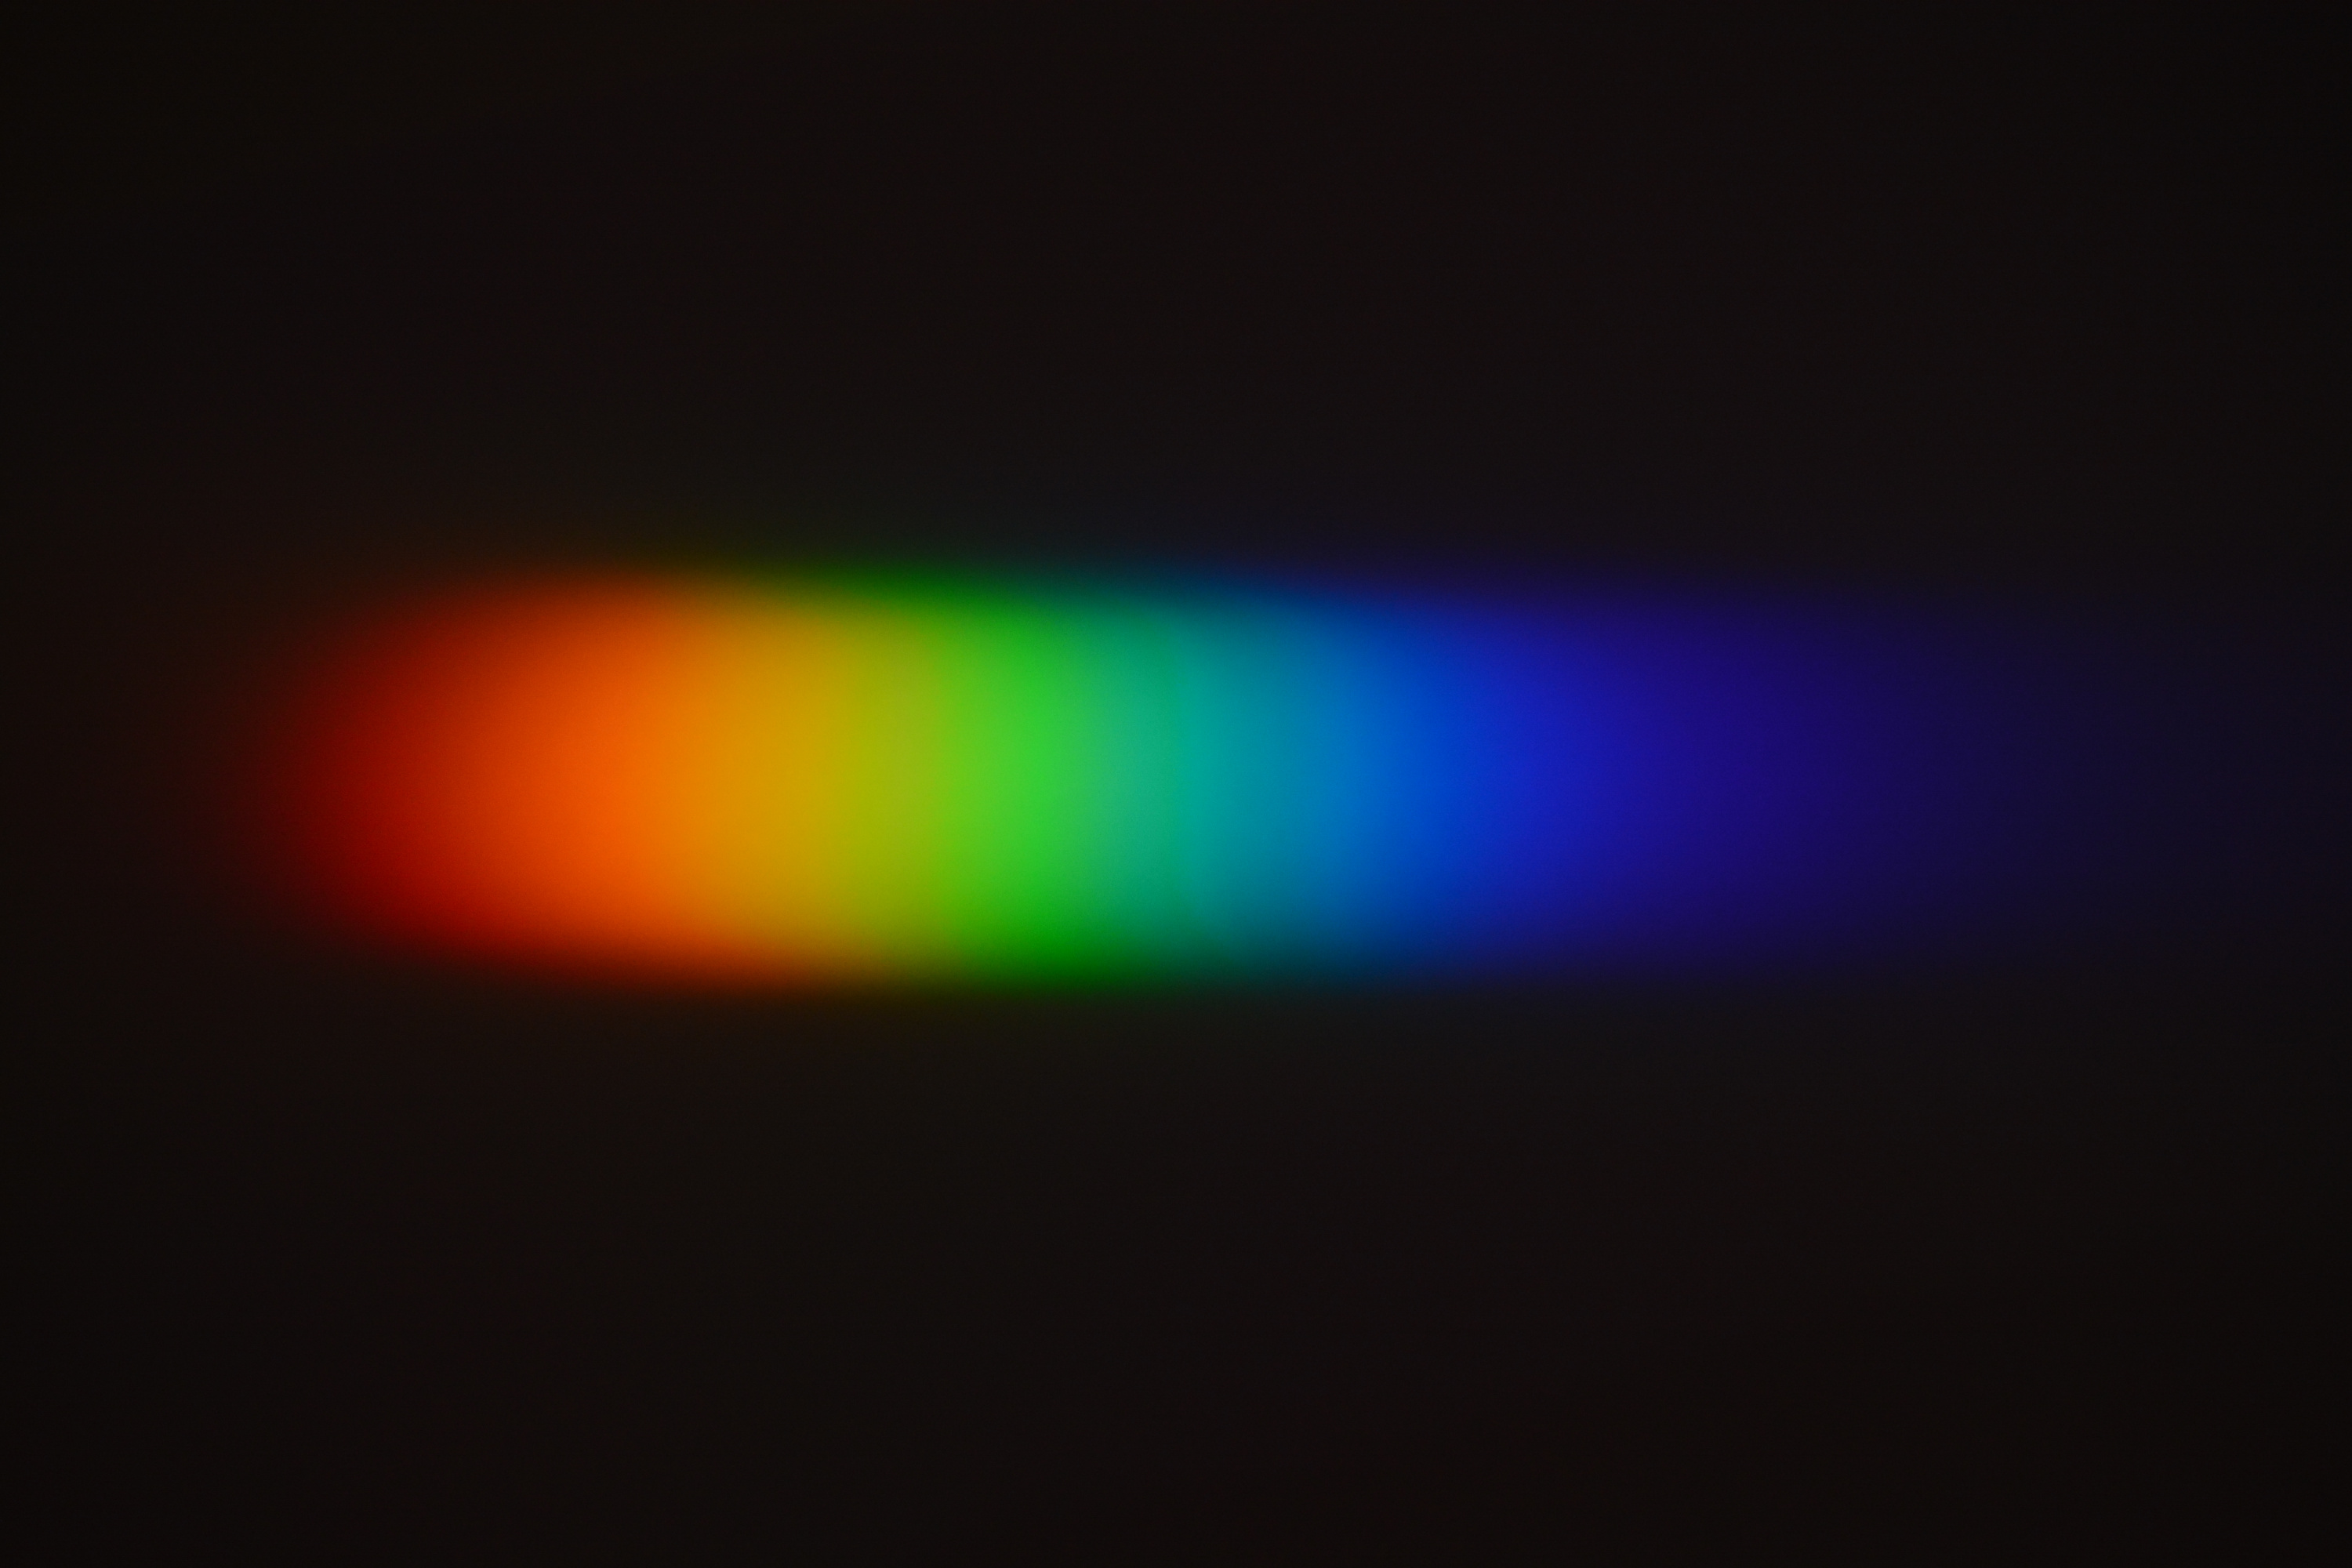
\includegraphics[width=7truecm]{slike/09_prizma.jpg}\hfill
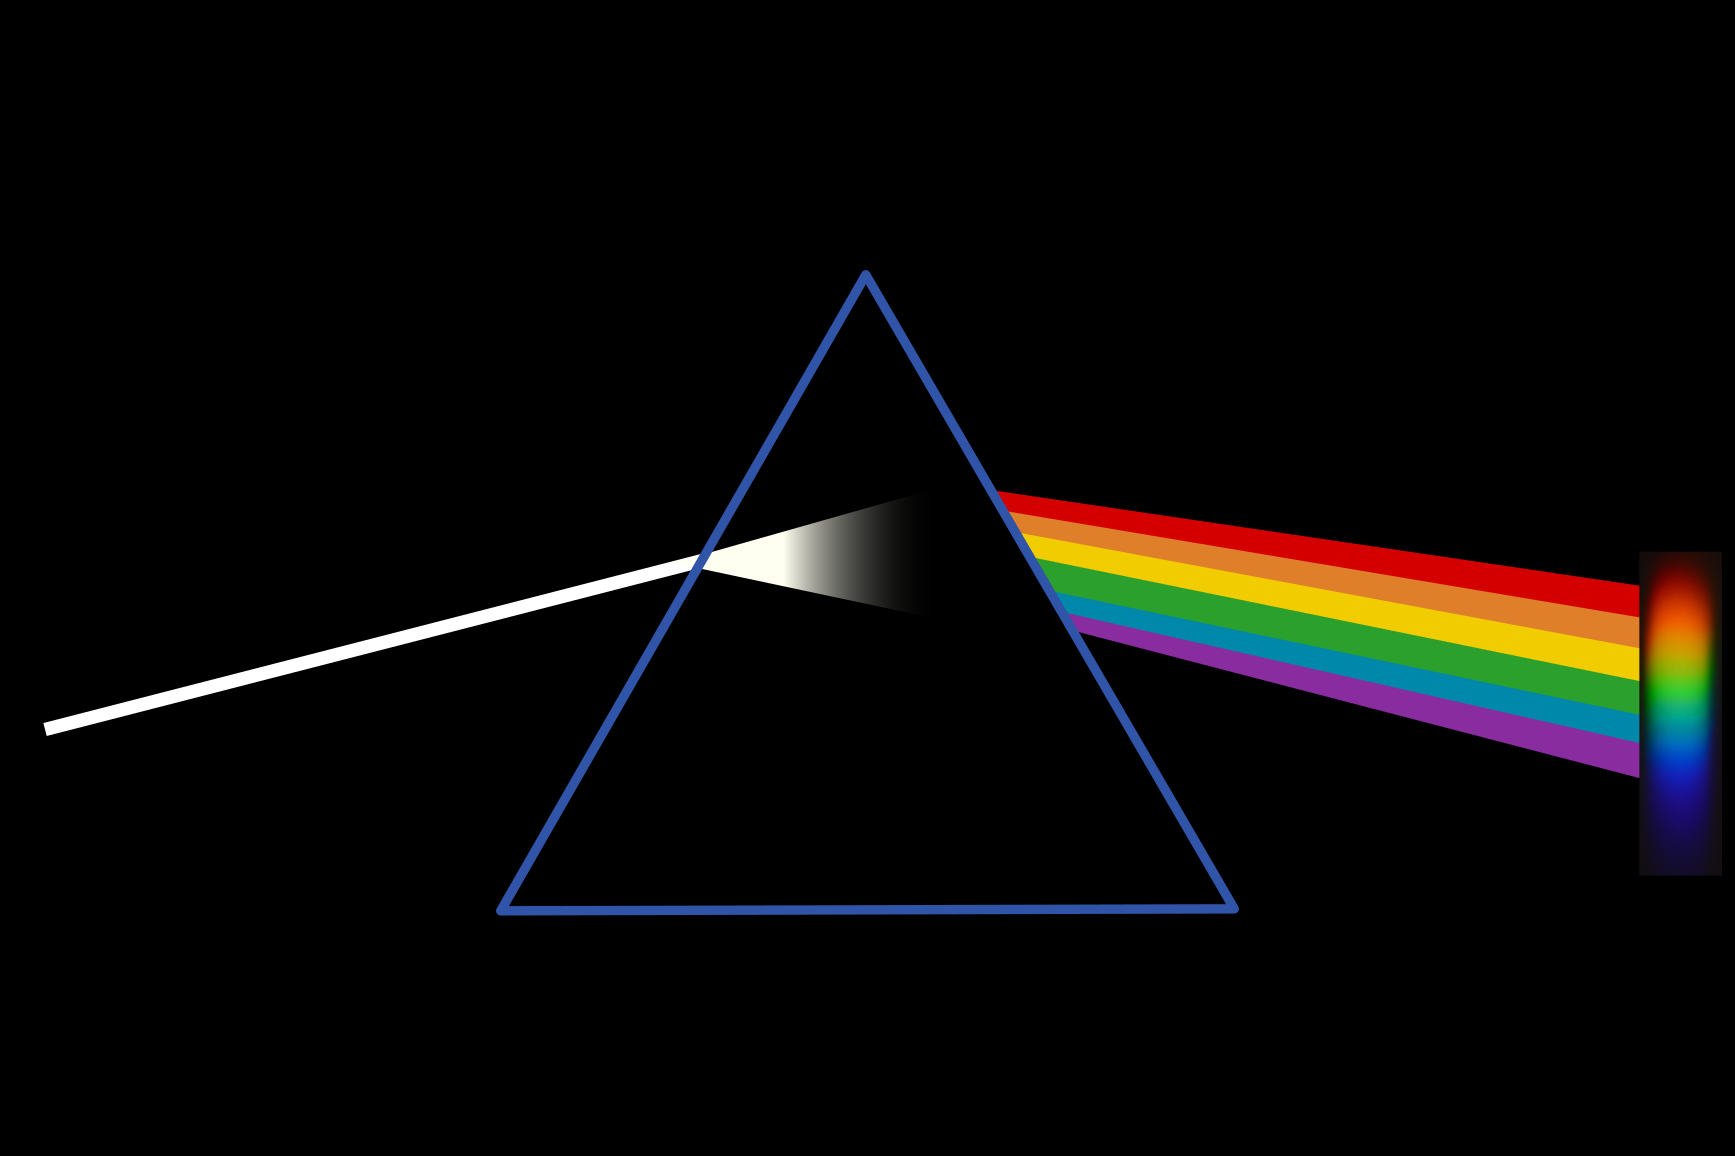
\includegraphics[width=7truecm]{slike/09_prizma_disp.png}
\caption{Razklon sončne (bele) svetlobe na prizmi: fotografija razklonjenega
snopa svetlobe (levo) in shematski prikaz učinka disperzije na prehod svetlobe
skozi prizmo (desno). Podobno sliko najdemo na naslovnici albuma 
{\it The Dark Side of the Moon} britanske zasedbe Pink Floyd.}
\label{fig:09_prizma}
\end{figure}
\vglue-2truemm
Drugi pomemben primer disperzije je mavrica, ki nastane zaradi
disperzije v dežnih kapljicah vode. Ko bela svetloba s Sonca vpade
na kapljice v zraku, se svetloba različnih valovnih dolžin 
lomi pod različnimi koti. Po odboju na zadnji strani kapljice 
zato različne barve svetlobe izhajajo iz kapljic pod različnimi koti, 
kar vidimo kot mavrico.
\begin{figure}[ht]
\centering
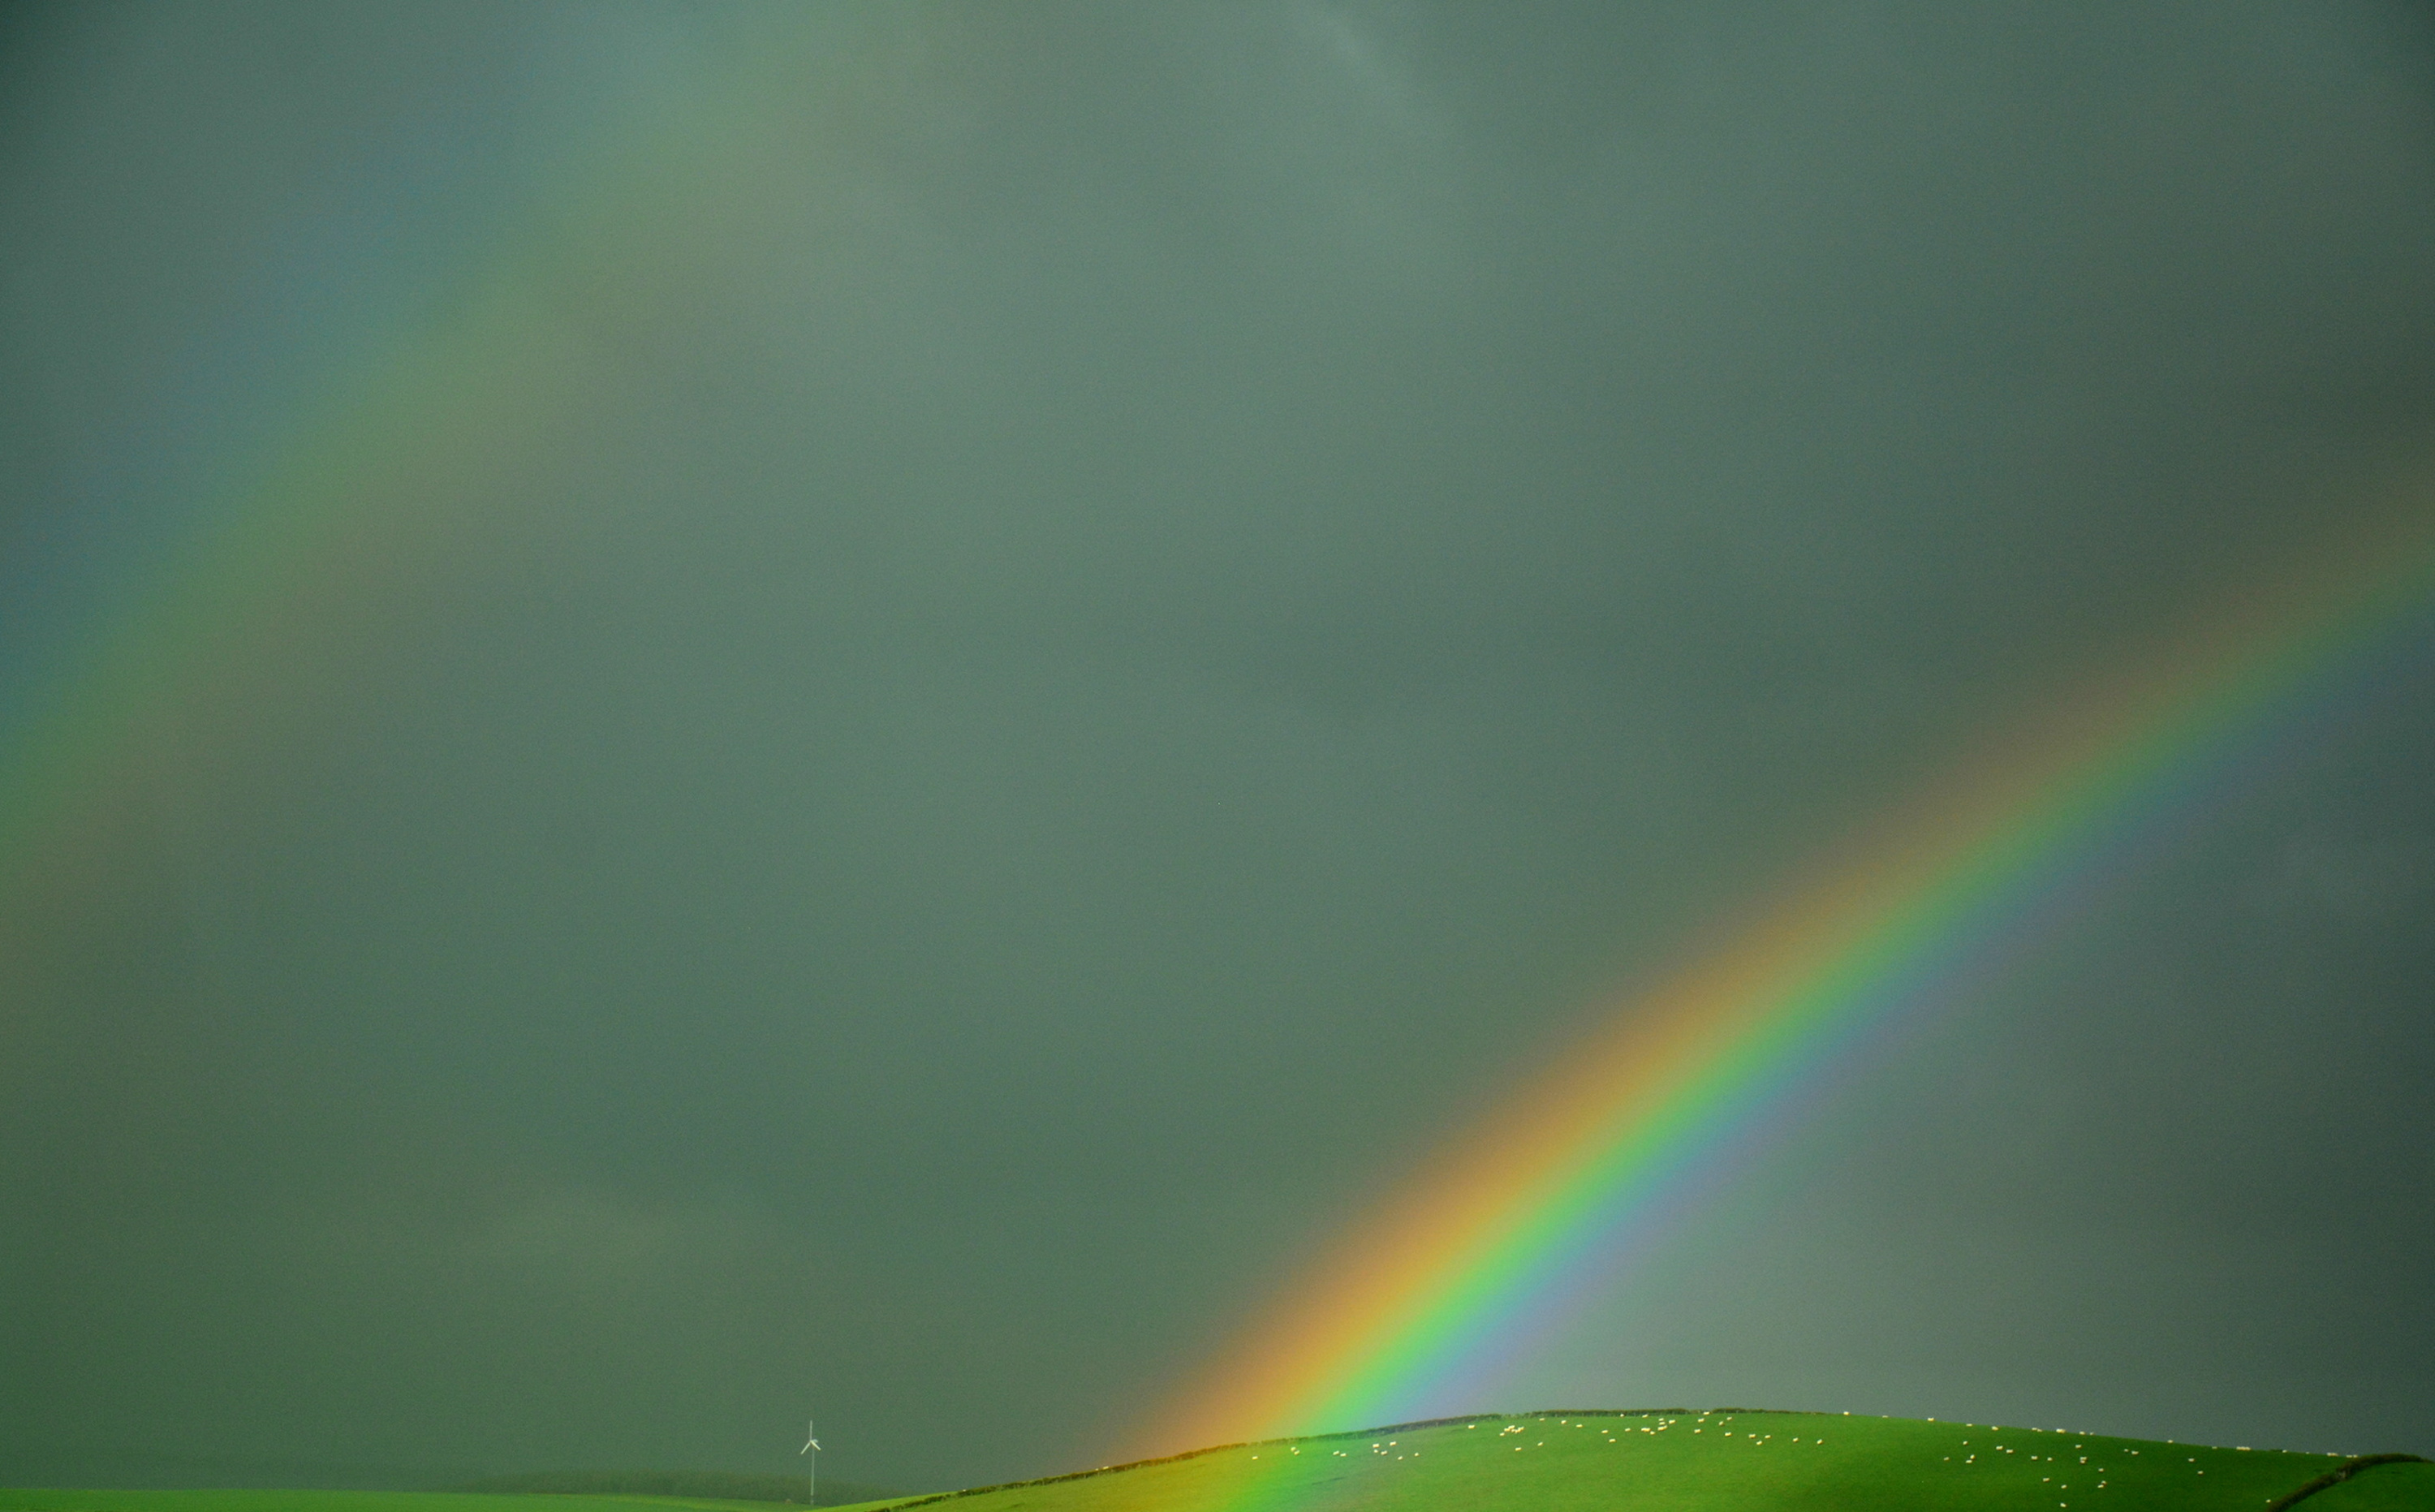
\includegraphics[width=7truecm]{slike/09_mavrica_photo.jpg}\hfill
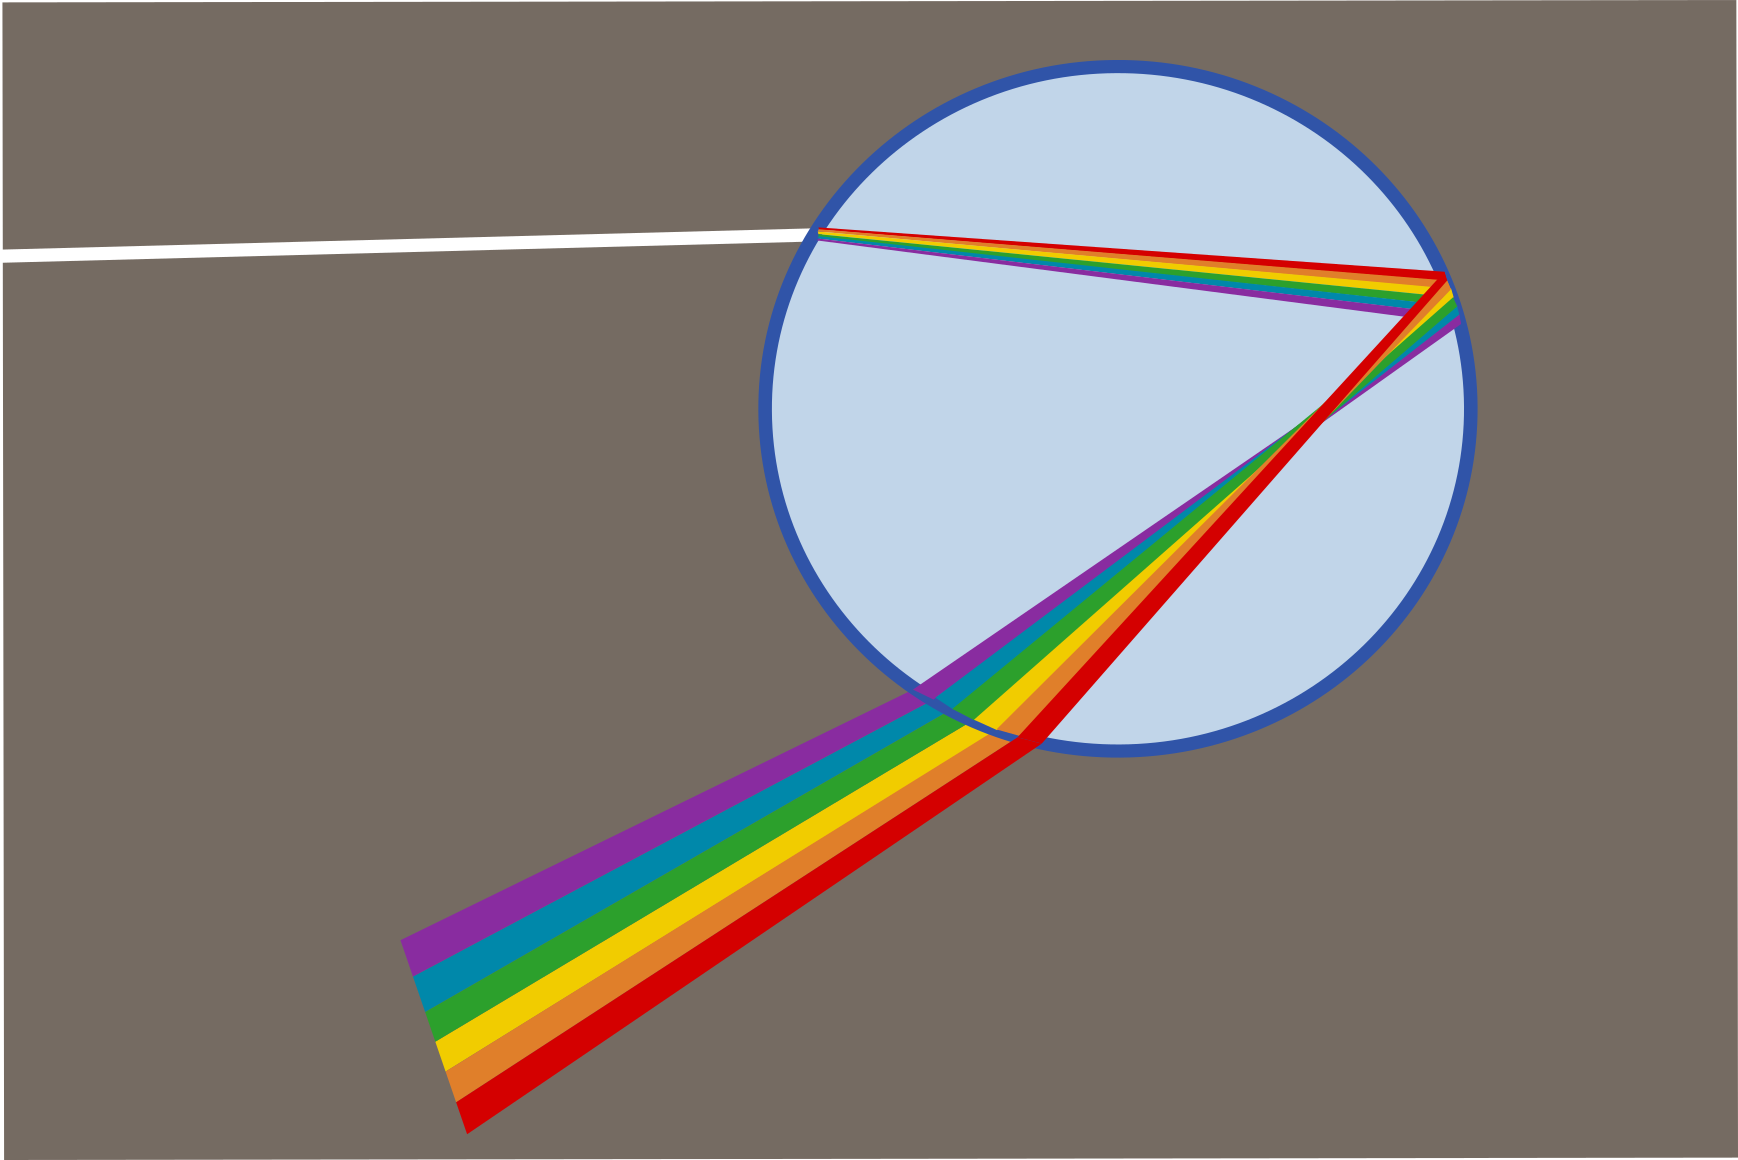
\includegraphics[width=7truecm]{slike/09_mavrica_disp.png}
\caption{Fotografija mavrice (levo) in shematski prikaz nastanka
mavrice (desno). Mavrica prvega reda (notranji kolobar) nastane ob enkratnem
odboju svetlobe v kapljici, mavrica drugega reda (zunanji kolobar) pa z dvakratnim, 
zato je vrstni red barv v njej obrnjen glede na mavrico prvega reda. 
Mavrica prvega reda se pojavi pri 
kotih okoli $41$--$42\si{\degree}$ glede na vpadno svetlobo, mavrica drugega
reda pa pri okoli $50$--$53\si{\degree}$. Med obema mavricama je značilen 
temnejši pas, tako imenovan Aleksandrov pas, po starogrškem mislecu Aleksandru
Afrodizijskem ($\sim 200$).}
\label{fig:09_mavrica}
\end{figure}
\end{example}

\begin{example}{\bf Kromatična aberacija leče.} Še en zanimiv primer 
disperzije opazimo pri preslikavi z lečo. 
Spoznali smo, da je goriščna razdalja leče odvisna
od lomnega količnika snovi, iz katere je leča narejena 
(enačba~\ref{eq:goriscna}). Zaradi disperzije stekla
je goriščna razdalja za različne valovne dolžine različna,
kar pripelje do napake leče, imenovane kromatična
aberacija. Na sliki je to opazno predvsem 
ob robovih slike, kjer so slike videti barvno razmazane. 
Napako zbiralne leče navadno odpravimo z dodatno razpršilno lečo, ki kompenzira
disperzijo prve leče. Nastali sestav imenujemo akromatska leča.
\begin{figure}[h!]
\vglue-3truemm
\centering
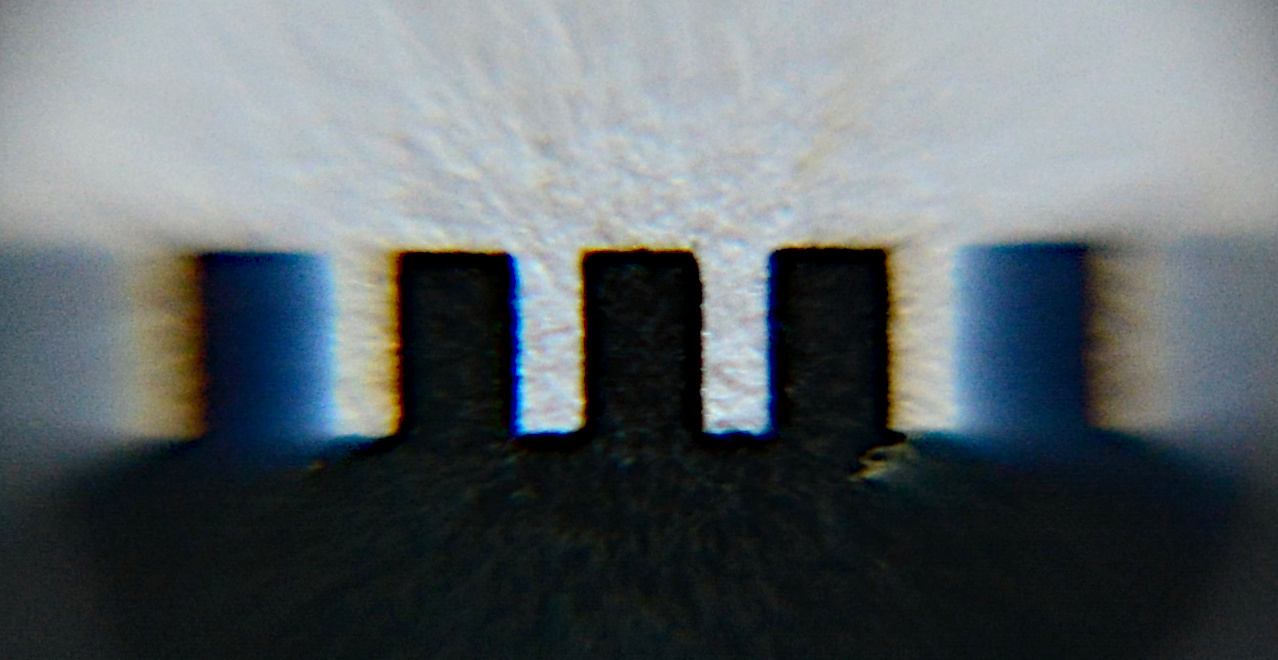
\includegraphics[width=6truecm]{slike/09_aberacija.jpg}
\caption{Slika je v sredini močne zbiralne leče ostra, ob robovih pa
se vidi učinek disperzije: modri odtenki so premaknjeni proti sredini 
leče, rdeči odtenki pa proti robu.}
\label{fig:09_aberacija}
\vglue-7truemm
\end{figure}

\end{example}

\begin{example}{\bf Disperzija v optičnih vlaknih.}
Disperzija igra zelo pomembno vlogo pri prenosu signalov
po optičnih vlaknih. Informacija po vlaknih potuje
v obliki kratkih sunkov svetlobe, ki imajo neko
končno spektralno širino. Posamezne spektralne 
komponente sunkov svetlobe zaradi disperzije 
potujejo z malenkost različnimi hitrostmi in sunki se 
med prehodom skozi vlakno podaljšajo. Ko je podaljšanje
tako veliko, da posameznih sunkov ne razločimo več, 
se informacija izgubi.  
Disperzija v optičnih vlaknih tako omejuje količino 
podatkov, ki jih lahko po vlaknu prenašamo v časovni enoti.
\begin{figure}[ht]
\centering
\def\svgwidth{130truemm} 
\input{slike/09_disperzija.pdf_tex}
\caption{Kratki sunki, ki vstopajo v optično vlakno, se zaradi 
disperzije podaljšajo. Kadar je disperzija premočna, sunkov
na izhodu ne zaznavamo več ločeno in informacija se izgubi.}
\label{fig:09_disperzijafib}
\end{figure}

\end{example}

\section{Prevodne snovi}
Potovanje svetlobe po prevodni snovi smo deloma že spoznali v 
razdelku~\ref{section:35}, ko smo zapisali valovno enačbo 
v prevodnih snoveh in izračunali lomni količnik.
V naslednjem poglavju (razdelek~\ref{section:410}) 
smo obravnavali odboj na prevodni snovi, zdaj pa si oglejmo odvisnost
lomnega količnika kovin od valovne dolžine vpadne svetlobe v mikroskopskem
modelu.

Obravnavajmo elektrone po Drudejevem modelu prostega elektronskega plina
v mreži nepremičnih pozitivnih nabojev. V tem modelu so elektroni prosti,
zato je konstanta vzmeti $k=0$ in lastna frekvenca $\omega_0=0$. Izhajamo 
iz splošne enačbe za izračun kompleksnega lomnega količnika $\mathcal{N}$
(enačba~\ref{eq:09_16}) in dobimo:
\beq
\mathcal{N}^2 = 1 + \frac{\omega_p^2}{-\omega^2 -i \gamma \omega} = 1- 
\frac{\omega_p^2}{\omega^2+i\gamma \omega}.
\label{eq:09_36}
\eeq
Pri tem smo z $\omega$ označili krožno frekvenco vpadne svetlobe, z
$\omega_p$ pa plazemsko frekvenco, podano z enačbo~(\ref{eq:09_14}). 
Koeficient dušenja $\gamma$ opisuje električno upornost, ki jo v idealnih 
prevodnikih lahko zanemarimo. Lomni količnik potem izračunamo kot:
\boxeq{eq:09_36a}{
n \approx \sqrt{1- \frac{\omega_p^2}{\omega^2}}.
}
Za vrednosti $\omega < \omega_p$ je lomni količnik imaginaren in svetloba se v snovi
močno absorbira. Po drugi strani je za krožne frekvence $\omega > \omega_p$ lomni količnik realen 
in snov prozorna. Ključni parameter pri odzivu prevodnikov je tako plazemska frekvenca. 

Plazemska frekvenca za srebro je v ultravijoličnem delu spektra 
pri okoli $320~\si{\nano\meter}$, za zlato pa pri okoli $500~\si{\nano\meter}$.
Lomni količnik srebra je tako za celoten spekter vidne svetlobe imaginaren in odbojnost
vidne svetlobe je približno enaka za vse valovne dolžine. Pri zlatu je lomni 
količnik za del vidnega spektra z daljšimi valovnimi dolžinami realen, pri 
krajših valovnih dolžinah pa je imaginaren. Rdeča in rumena barva se zato v zlatu 
ne moreta razširjati in ko bela svetloba vpade na zlato, se rdeča in rumena svetloba
od njega odbijeta. To da zlatu značilno rdečkasto-rumeno barvo. Za modre odtenke
svetlobe je lomni količnik zlata realen, zato se modri odtenki znatno šibkeje odbijajo od površine.
\begin{figure}[ht]
\centering
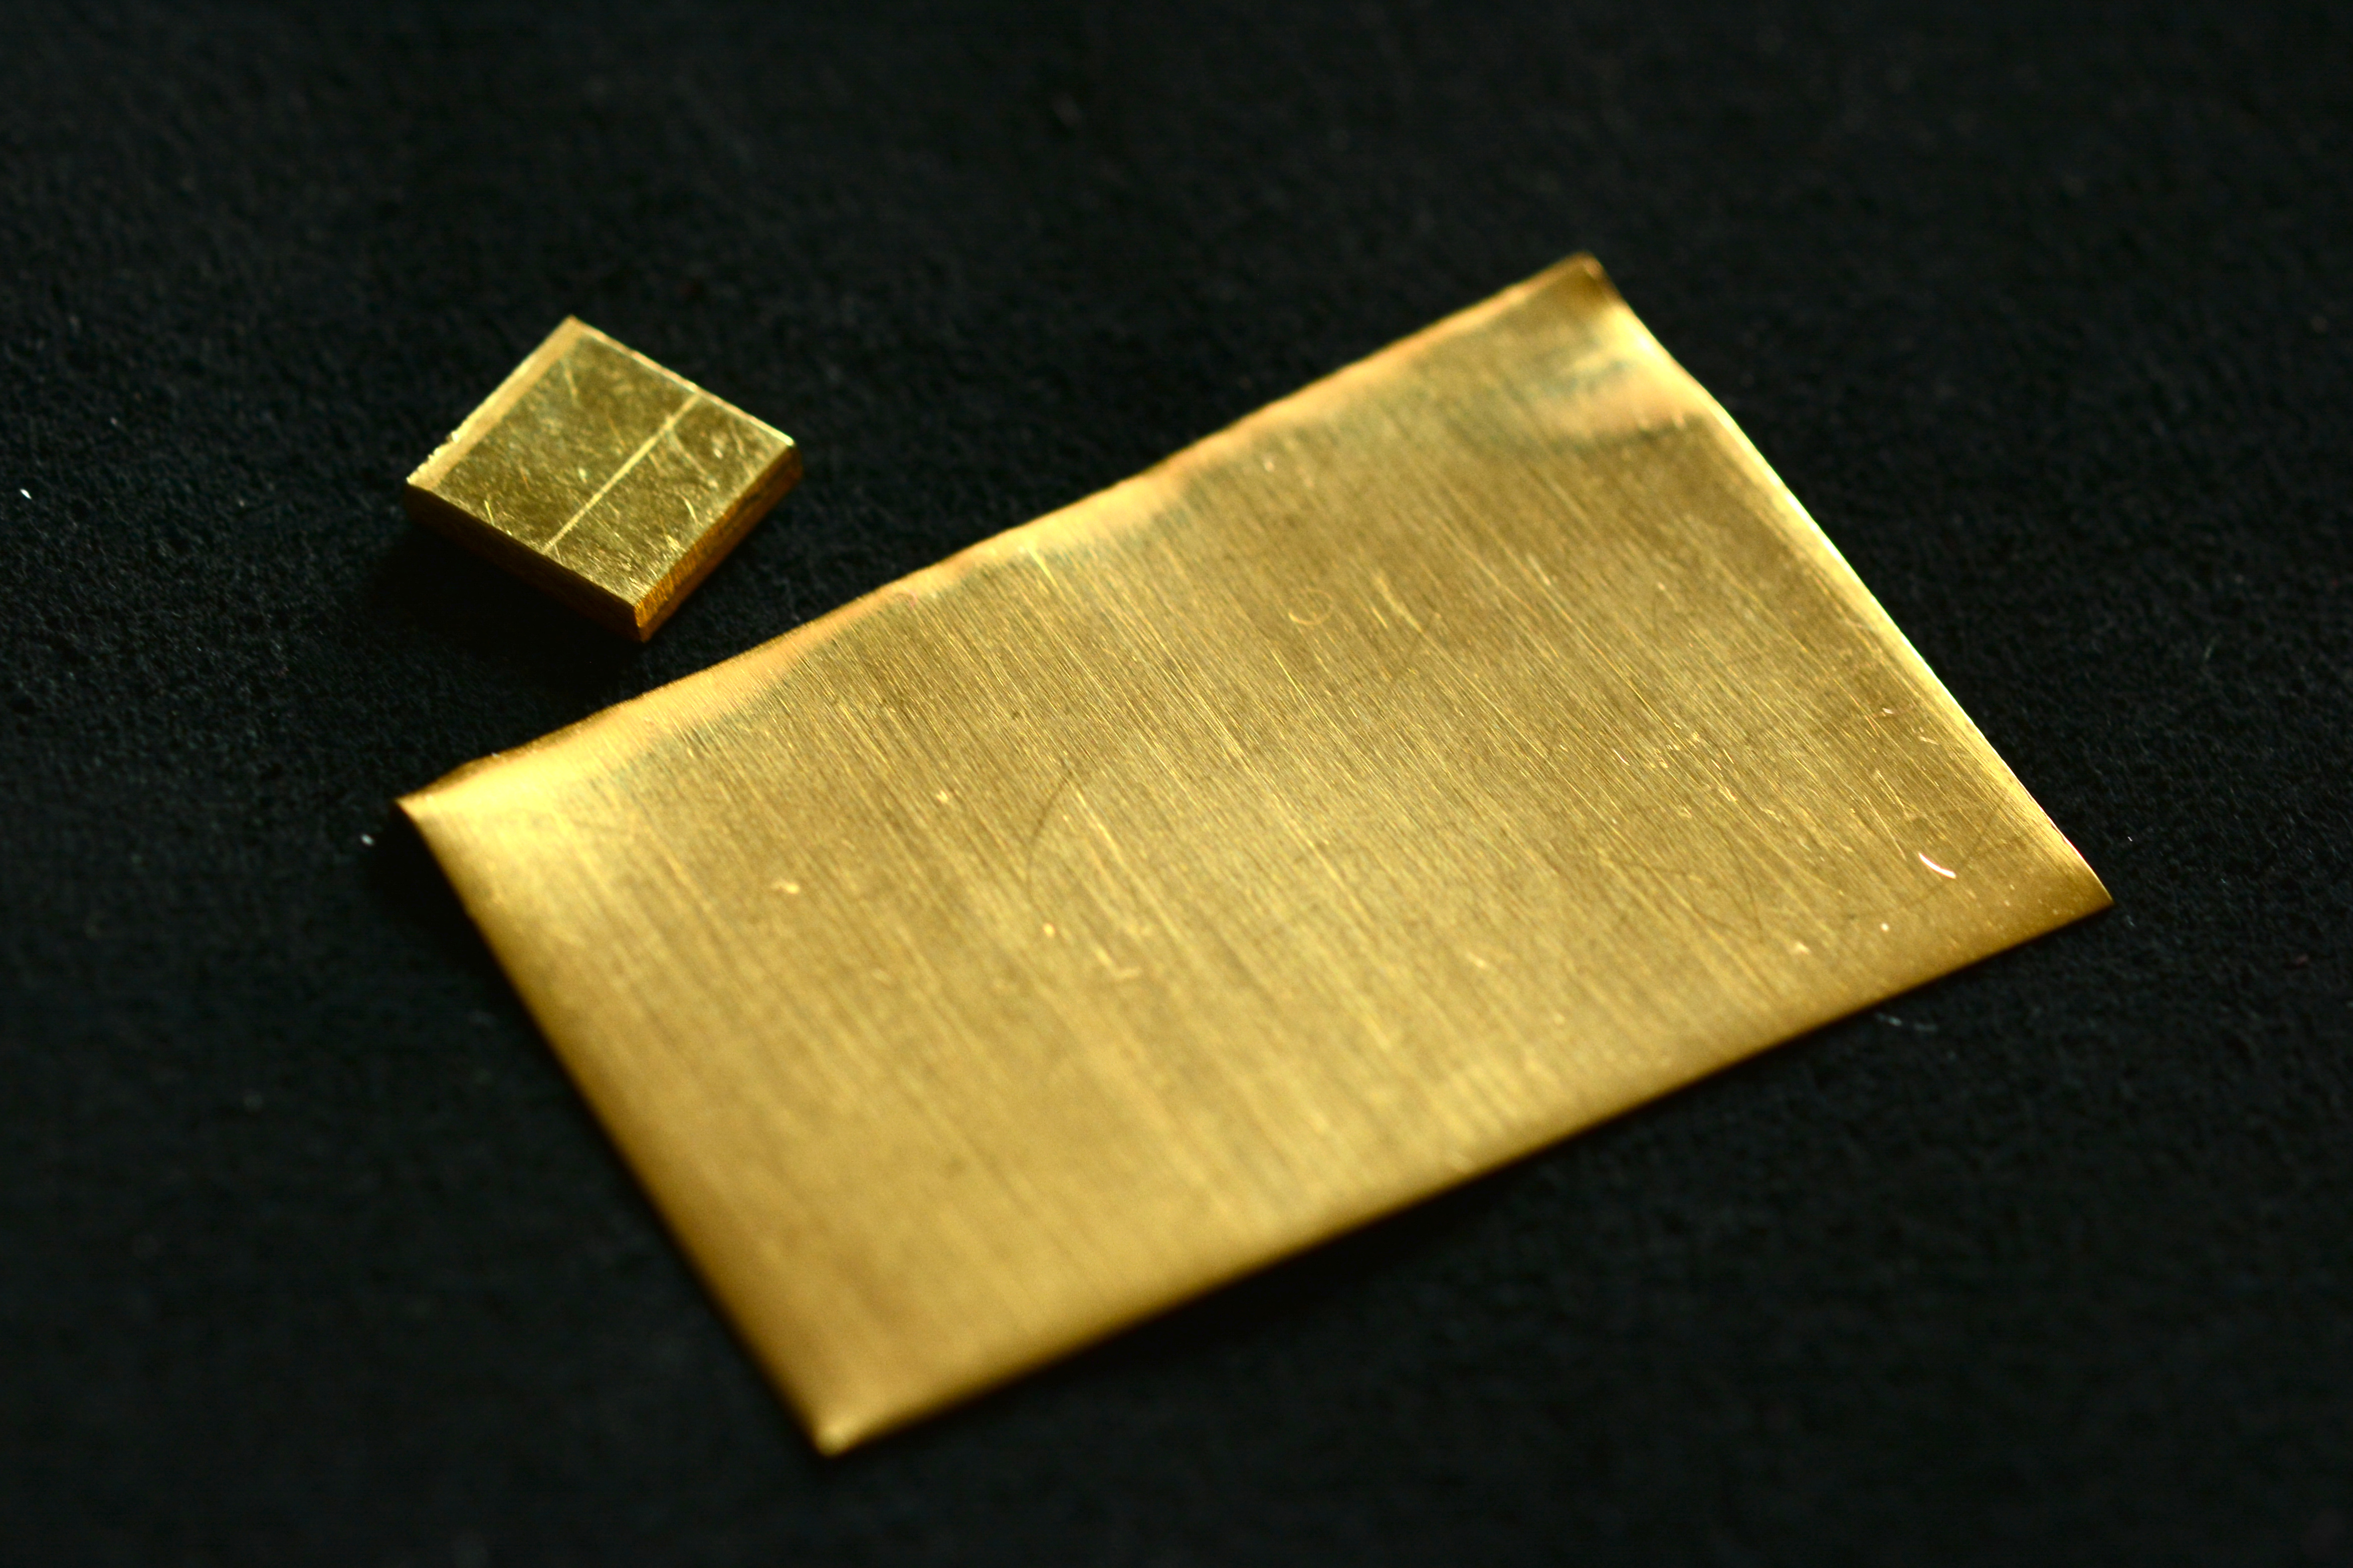
\includegraphics[width=7truecm]{slike/09_zlato.jpg}\hfill
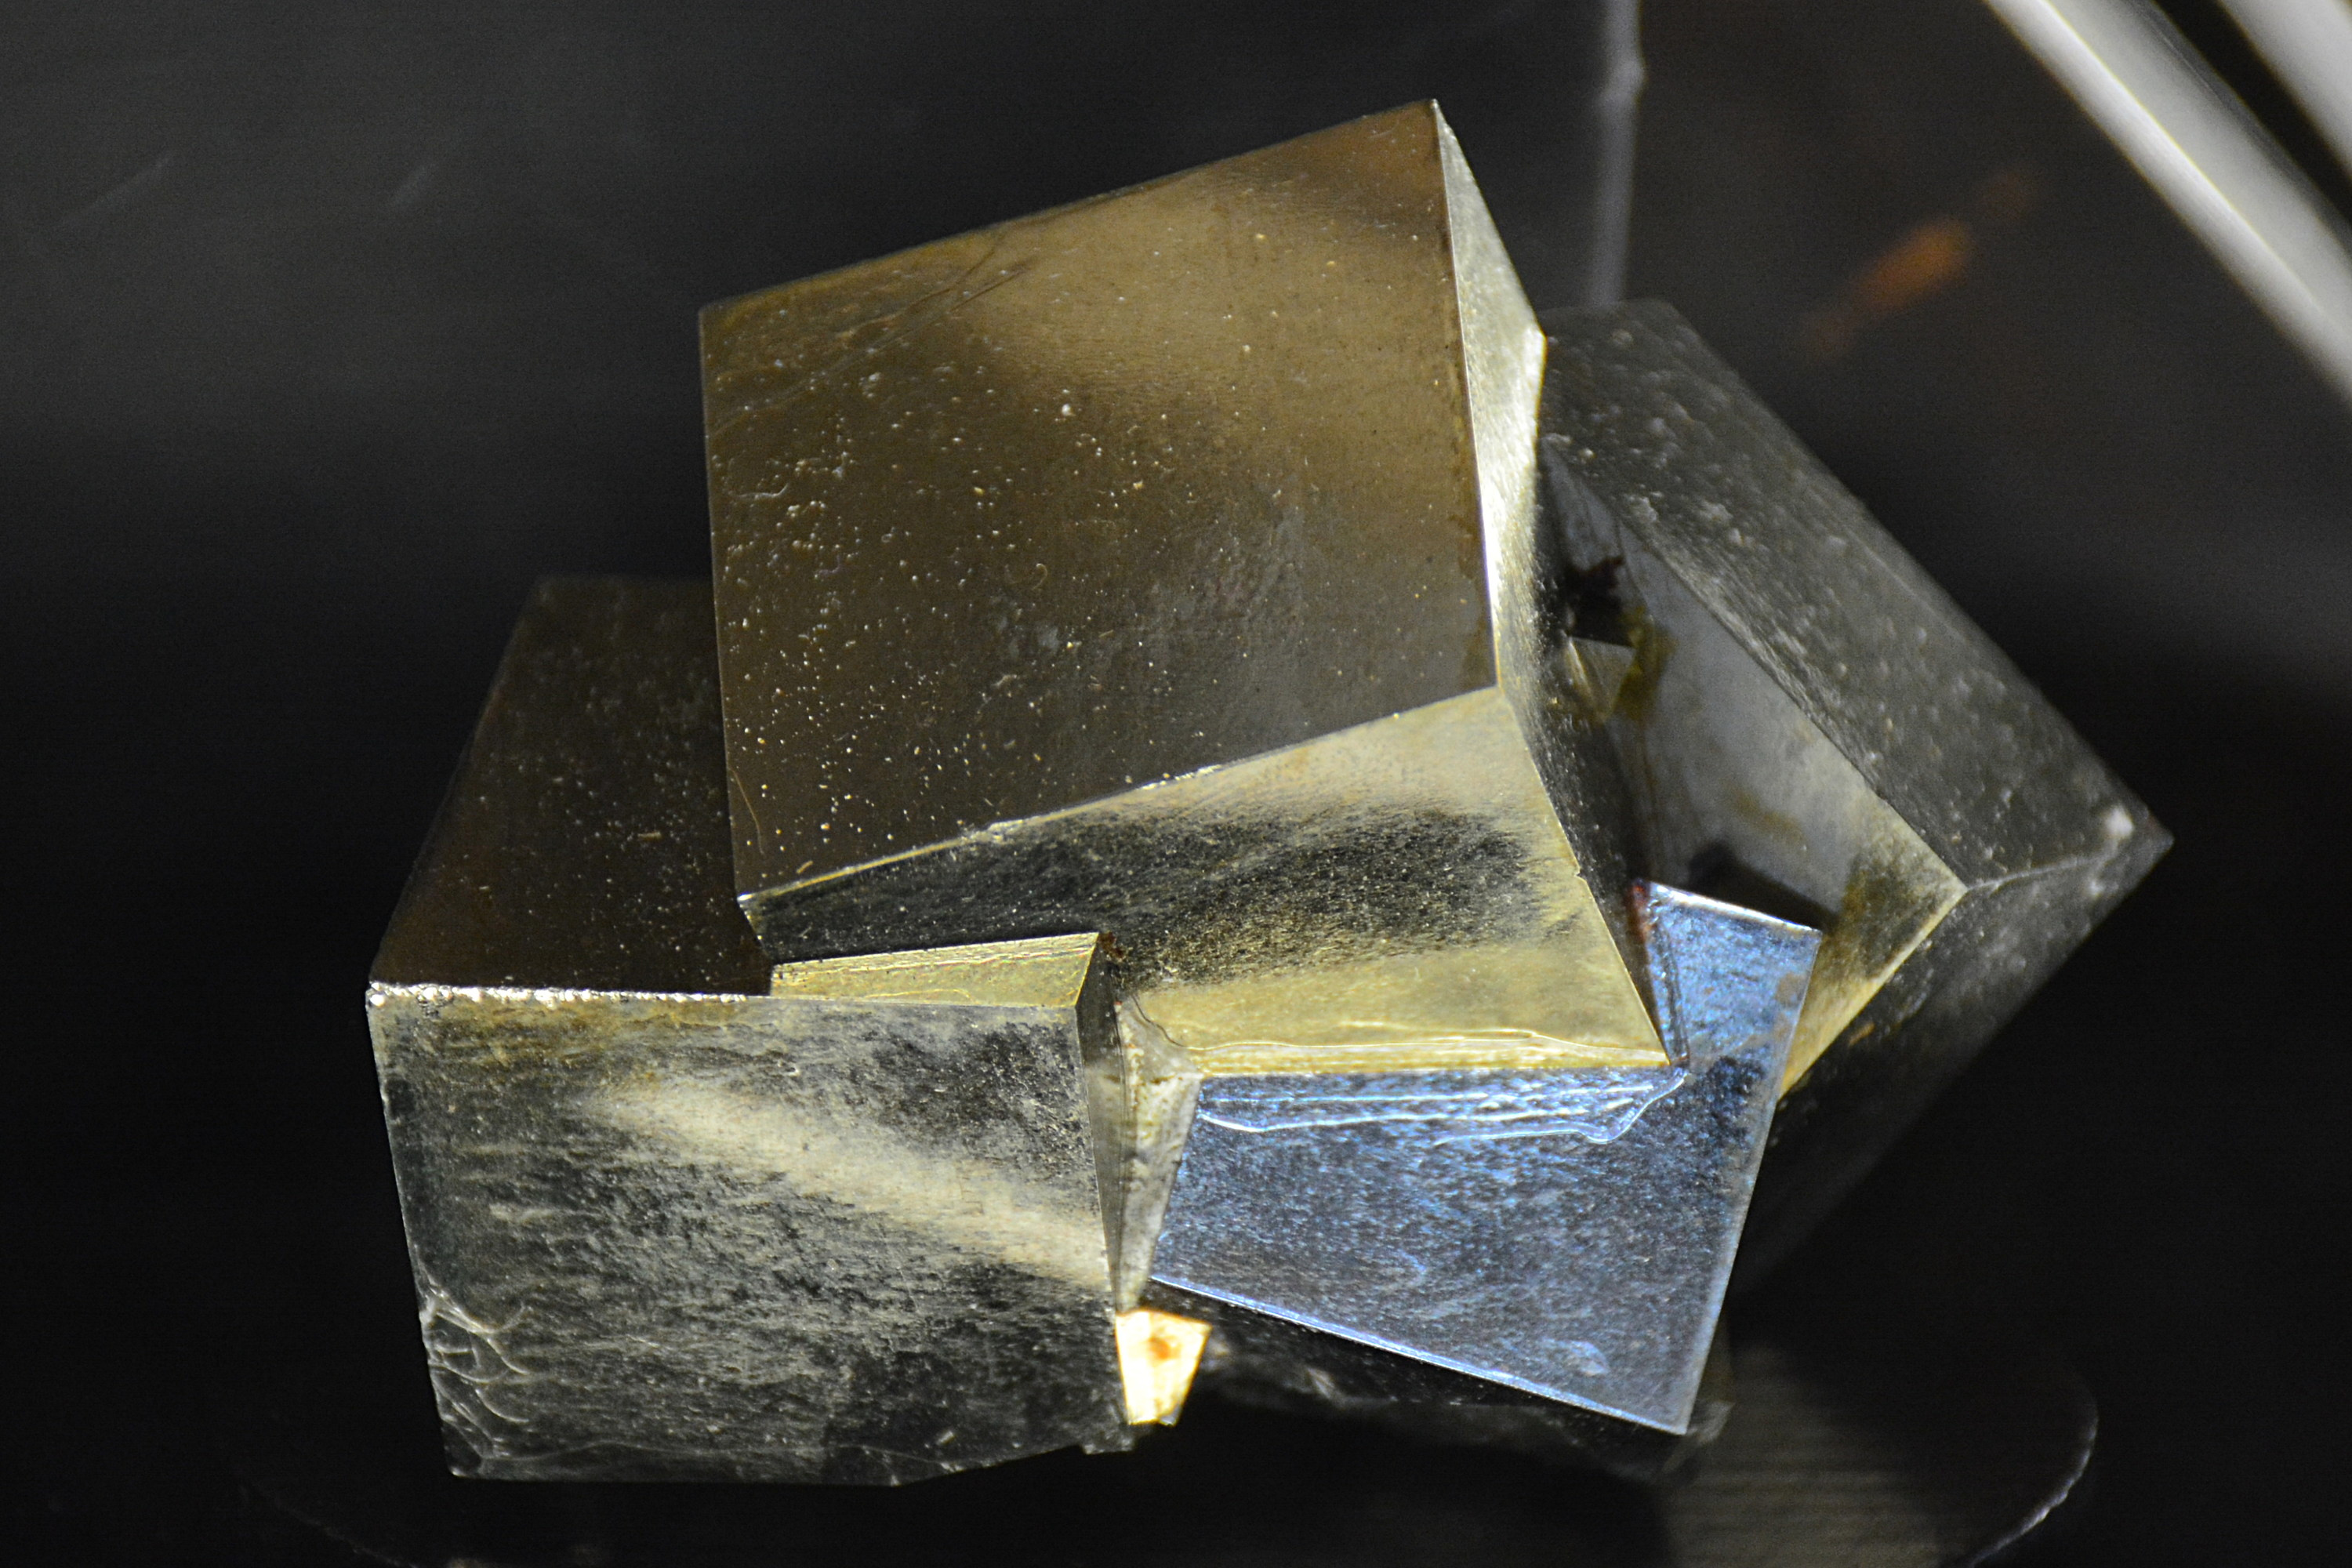
\includegraphics[width=7truecm]{slike/09_pirit.jpg}
\caption{Ploščica $91,6\%$ (22-karatnega) in košček $83,3\%$ (20-karatnega) zlata (levo). 
Podobno zlatorumeno barvo ima tudi pirit FeS$_2$ (desno).}
\label{fig:09_zlato}
\end{figure}
\begin{figure}[h!]
\centering
\def\svgwidth{100truemm} 
\input{slike/09_kovine.pdf_tex}
\caption{Odbojnosti na kovinah v odvisnosti od valovne dolžine vpadne svetlobe. Odbojnost
srebra je v vidnem delu spektra (osenčeno področje) praktično 
neodvisna od valovne dolžine, podobno velja tudi za aluminij, zato sta kovini
videti neobarvano. Odbojnosti bakra in zlata sta pri modrih odtenkih bistveno 
manjši kot pri rdečih in rumenih, zato ima baker značilno rdečkasto barvo in zlato
rumeno-rdečkasto barvo (Povzeto po E. Hecht, {\it Optics}, Pearson, 2017.)}
\label{fig:09_kovine}
\end{figure}
\begin{figure}[h!]
\centering
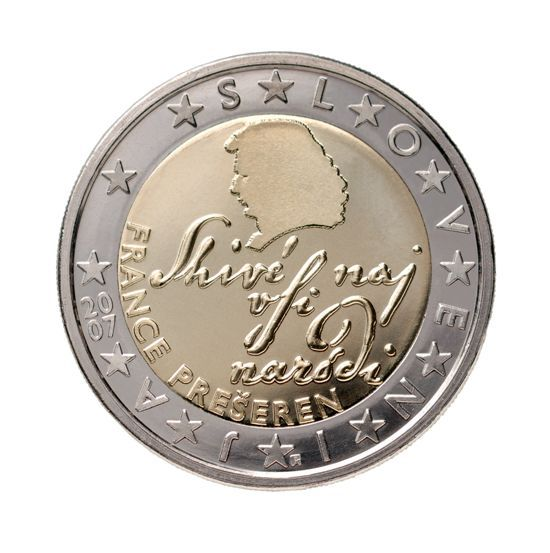
\includegraphics[width=35truemm]{slike/09_2euro.jpg}
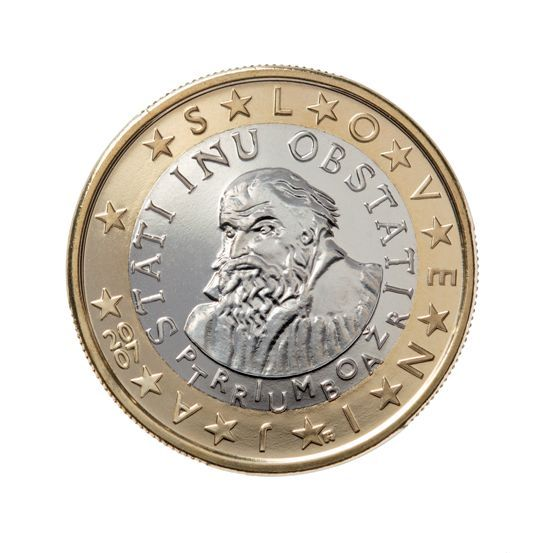
\includegraphics[width=35truemm]{slike/09_1euro.jpg}
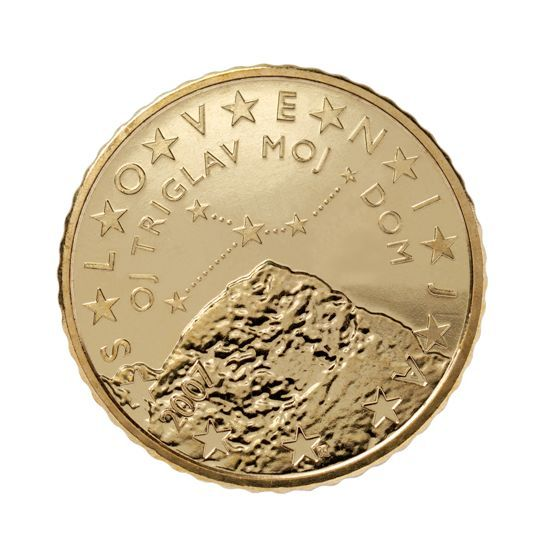
\includegraphics[width=35truemm]{slike/09_50centov.jpg}
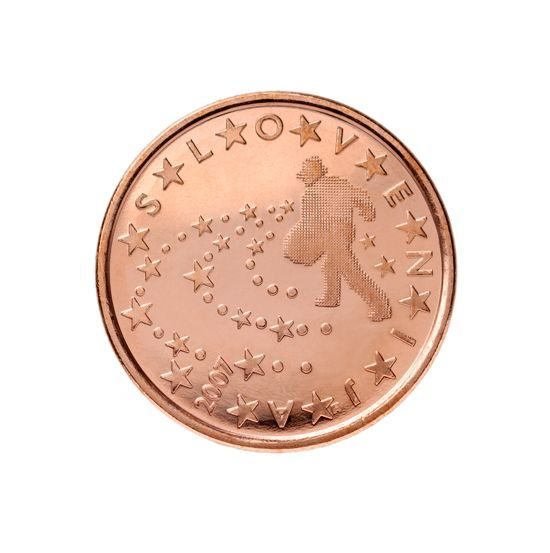
\includegraphics[width=35truemm]{slike/09_5centov.jpg}
\caption{Evrski kovanci so različnih barv, saj so narejeni iz različnih zlitin. Kovanec za 2~€ je 
ob robu iz zlitine bakra in niklja, osrednji del pa je triplastna struktura nikelj-medenina, nikel, nikel-medenina. Kovanec za 1~€ je ob robu zlitina nikelj-medenina, osrednji del pa triplastna struktura
nikel-baker, nikel, nikel-baker. Kovanec za 50~centov je iz tako imenovanega nordijskega 
zlata ($89\%$ bakra, $5\%$ aluminija, $5\%$ cinka in $1\%$ kositra), kovanec za 5~centov pa je iz jekla, prevlečenega z bakrom. Z različnimi zlitinami lahko tako dosežemo ``zlat'' videz kovancev, medtem ko
je čisti baker izrazito rdečkaste barve (Foto: Banka Slovenije).}
\label{fig:09_kovanci}
\end{figure}


\section{Optični metamateriali}
Posebna vrsta snovi so metamateriali. To so snovi, ki jih v naravi ne najdemo (so umetno
ustvarjene), zaradi svoje natančno načrtovane in zapletene strukture pa delujejo na 
vpadno elektromagnetno valovanje drugače od navadnih snovi. Za optiko so najbolj zanimivi
metamateriali, ki imajo na določenem frekvenčnem območju negativni lomni količnik.

V tretjem poglavju smo spoznali, da je lomni količnik enak korenu dielektričnosti
(enačba~\ref{eq:n}). Rezultat izhaja iz zveze $n^2 = \varepsilon \mu$, pri čemer smo 
vzelo pozitivno vrednost korena. Druga rešitev, sicer precej bolj nenavadna, je negativna
vrednost lomnega količnika $n = - \sqrt{\varepsilon \mu}$. To lahko dosežemo pri snoveh,
za katere sta na določenem frekvenčnem območju hkrati $\varepsilon<0$ in $\mu<0$. 
Ker je njun produkt pozitiven, se svetloba v snovi ne absorbira, njen lomni količnik 
pa je negativen. V navadnih snoveh tako velja:
\beq
\varepsilon >0, \mu > 0 \qquad \Rightarrow \qquad n^2 = \varepsilon \mu 
\qquad \Rightarrow \qquad n = \sqrt{\varepsilon\mu},
\label{eq:09_37m}
\eeq
v metamaterialih pa:
\beq
\varepsilon <0, \mu < 0 \qquad \Rightarrow \qquad n^2 = \varepsilon \mu 
\qquad \Rightarrow \qquad n = -\sqrt{\varepsilon\mu}<0. 
\label{eq:09_38}
\eeq
Metamaterialov v naravi ne najdemo, lahko pa jih za izbrane valovne dolžine naredimo z
nanostrukturiranimi kompozitnimi materiali. Pri tem mora biti sestavni element kompozita
bistveno manjši od valovne dolžine vpadne svetlobe, zato metamateriali tipično delujejo v 
mikrovalovnem območju spektra.

V metamaterialih je posebej zanimiv lom svetlobe. Zapišemo lomni zakon 
(enačba~\ref{eq:lomnizakon}):
\beq
n_1 \sin\alpha = n_2 \sin\beta,
\label{eq:09_39}
\eeq
pri čemer velja $n_1>0$ in $n_2<0$. Ko svetloba vpade na metamaterial pod vpadnim
kotom $\alpha>0 $, je lomni kot $\beta <0$. 
\begin{figure}[h]
\centering
\def\svgwidth{80truemm} 
\input{slike/09_meta.pdf_tex}
\caption{Lom svetlobe ob prehodu iz navadne snovi v metamaterial z negativnim lomnim
količnikom. V metamaterialu sta smeri energijskega toka $\mathbf{S}$ 
in valovnega vektorja $\mathbf{k}$ nasprotni.}
\label{fig:09_meta}
\end{figure}

Drugo zanimivo lastnost  metamaterialov spoznamo, če si ogledamo Poyntingov vektor. 
Spomnimo se (enačba~\ref{eq:Poyntingov}), da velja zveza 
$\mathbf{S} = \mathbf{E}\times \mathbf{H}$. Smer Poyntingovega vektorja določa smer
energijskega toka in v navadnih snoveh je ta smer enaka smeri valovnega vektorja.
V metamaterialih pa negativna vrednost konstant učinkuje enako, kot bi učinkovala
sprememba predznaka magnetnega polja. Iz zveze za Poyntingov vektor sledi, da ima
smer energijskega toka v metamaterialih nasprotno smer od smeri valovnega vektorja. 

\section{Optična aktivnost}
Določene snovi imajo prav posebno sposobnost sukanja polarizacije vpadne svetlobe.
Take snovi imenujemo optično aktivne snovi, pojav sukanja linearne polarizacije
vpadne svetlobe ob prehodu skozi snov pa optična aktivnost.
Optične aktivno snovi so kiralne, torej brez zrcalne simetrije, in so lahko
v trdnem, tekočem ali plinastem stanju. Primeri optično aktivnih snovi
so raztopine glukoze in fruktoze, aminokisline ter kremen.

Naj na optično aktivno snov v smeri osi $z$ 
vpada svetloba, ki je linearno polarizirana vzdolž osi $x$ 
(slika~\ref{fig:09_aktivnost}). Po 
prehodu skozi snov se smer linearne polarizacije
zasuče za kot $\Delta \varphi$ glede na os $x$, pri čemer je kot zasuka 
odvisen od snovi in od dolžine poti skozi snov $L$. Z Jonesovimi
vektorji vpadno polarizacijo v opisanem primeru zapišemo kot:
\beq
\mathbf{J}_{in} = 
\left[\begin{array}{c}
1\\
0\\
\end{array}\right]\!\!,
\label{eq:09_40}
\eeq
zasukano izhodno polarizacijo pa kot:
\beq
\mathbf{J}_{out} = 
\left[\begin{array}{c}
\cos \Delta \varphi\\
\sin \Delta \varphi\\
\end{array}\right]\!\!.
\label{eq:09_41}
\eeq
Gledano s stališča opazovalca (proti izvoru svetlobe)
snov polarizacijo zasuče v levo glede na prvotno smer, zato tako snov imenujemo
levosučna snov. Po dogovoru je kot zasuka za levosučne snovi negativen, za
desnosučne pa pozitiven.
\begin{figure}[h]
\centering
\def\svgwidth{100truemm} 
\input{slike/09_aktivnost.pdf_tex}
\caption{Optično aktivne snovi sučejo smer vpadne linearne polarizacije. Na sliki
je primer levosučne snovi, saj se po prehodu snovi polarizacija, gledano v smeri 
izvora svetobe, zasuče v levo.}
\label{fig:09_aktivnost}
\vglue-7truemm
\end{figure}
 
\begin{remark}
Optična aktivnost se v snoveh lahko pojavi zaradi vijačne kristalne strukture
(kot v kremenu) ali zaradi kiralnih molekul, ki snov sestavljajo (na primer sladkorji). 
Prvi mehanizem je vezan na točno določeno ureditev molekul, zato so 
take snovi optično aktivne le v kristalni obliki. Staljen kremen, ki ob taljenju
izgubi vijačno strukturo, je optično neaktiven. Po drugi strani snovi, ki so 
optično aktivne zaradi kiralnih gradnikov, ostanejo optično aktivne, tudi 
če jih stalimo, raztopimo v vodi ali izparimo.

Za kiralne molekule je značilno, da njene zrcalne slike ne moremo dobiti z rotacijo
ali translacijo prvotne molekule, ampak je potrebna zrcalna preslikava. Asimetrija 
se pojavi zaradi razporeditve atomov okoli tako imenovanega kiralnega centra. Navadno
je to ogljikov atom, ki ima pripete štiri različne kemijske skupine.
Dve možni konformaciji molekule imenujemo optična izomera 
oziroma enantiomera, mešanico obeh izomerov v razmerju 50:50 pa
racemat. Racemat je optično neaktiven.

Čeprav sta si izomera neke snovi zelo podobna in imata enako molekulsko formulo, 
je razlika med njima ključna. Tako so vse standardne aminokisline razen
glicina optično aktivne in brez izjeme vse levosučne. Po drugi strani je skoraj 
vsa glukoza v naravi desnosučna, prav tako tudi drugi enostavni sladkorji. Problem
nastane pri umetni sintezi spojin, saj med kemijskimi reakcijami praviloma
nastajata oba izomera v enaki količini. Če želimo nastale spojine uporabiti, na
primer v farmaciji, ju je treba ločiti, saj imata lahko izomera povsem različen
učinek: en zdravilen in drug škodljiv.
\end{remark}
\vglue-5truemm
\begin{figure}[h]
\centering
\def\svgwidth{60truemm} 
\input{slike/09_kiralna.pdf_tex}
\caption{Ena najpreprostejših stabilnih kiralnih molekul je bromoklorofluorometan. Zrcalne
slike molekule ne moremo dobiti z rotacijo ali translacijo prvotne, zato pravimo, 
da je molekula kiralna. Kiralni center je ogljik.}
\label{fig:09_kiralna}
\end{figure}

Sukanje linearne polarizacije v optično aktivnih snoveh preprosto pojasnimo
z različnima lomnima količnikoma za levo in desno krožno polarizirano valovanje\footnote{~Optično 
aktivnost zato imenujemo tudi cirkularni dvojni lom. Pri navadnem dvojnem lomu 
(glej poglavje~\ref{chap:AnizotropneSnovi}) se razlikujeta lomna količnika za dve 
ortogonalni linearni polarizaciji, pri cirkularnem dvojnem lomu pa se razlikujeta lomna
količnika za dve nasproti krožni polarizaciji.}.
Označimo desno cirkularno polarizacijo z D in levo z L. Snov je optično aktivna, če velja:
\boxeq{eq:09_42}{
n_D \neq n_L.
}
Linearno polarizirano valovanje zapišemo kot vsoto dveh cirkularno polariziranih
valovanj. Pred vpadom na snov je tako:
\beq
\mathbf{J}_{1} = 
\left[\begin{array}{c}
1\\
0\\
\end{array}\right] = 
\frac{1}{2}
\left[\begin{array}{c}
1\\
-i\\
\end{array}\right]
+ 
\frac{1}{2}
\left[\begin{array}{c}
1\\
i\\
\end{array}\right]\!\!.
\label{eq:09_43}
\eeq
Po prehodu skozi snov različno krožno polarizirani komponenti 
občutita različna lomna količnika in imata zato ob prehodu snovi z 
dolžino $L$ različni fazi:
\beq
\mathbf{J}_{2}  = 
\frac{1}{2}
\left[\begin{array}{c}
1\\
-i\\
\end{array}\right]e^{ik_0n_D L}
+ 
\frac{1}{2}
\left[\begin{array}{c}
1\\
i\\
\end{array}\right]e^{ik_0n_L L}.
\label{eq:09_44}
\eeq
Izraz preoblikujemo in dobimo:
\beq
\mathbf{J}_{2}  = \frac{1}{2} e^{ik_0n_D L/2}e^{ik_0n_L L/2}
\left(
\left[\begin{array}{c}
1\\
-i\\
\end{array}\right]e^{ik_0n_D L/2} e^{-ik_0n_L L/2}+
\left[\begin{array}{c}
1\\
i\\
\end{array}\right]e^{-ik_0n_D L/2} e^{ik_0n_L L/2}
\right)\!\!.
\label{eq:09_45}
\eeq
Vpeljemo povprečni lomni količnik $\overline{n} = (n_L + n_D)/2$ in razliko
med lomnima količnikoma $\Delta n = n_L-n_D$. Sledi:
\beq
\mathbf{J}_{2}  = \frac{1}{2} e^{ik_0\overline{n} L}
\left(
\left[\begin{array}{c}
1\\
-i\\
\end{array}\right]e^{-ik_0 \Delta n L/2}+
\left[\begin{array}{c}
1\\
i\\
\end{array}\right]e^{ik_0\Delta n L/2}
\right)\!\!.
\label{eq:09_46}
\eeq
Eksponenta izrazimo s kotnima funkcijama in dobimo:
\beq
\mathbf{J}_{2}  = \frac{1}{2} e^{ik_0\overline{n} L}
\left[\begin{array}{c}
2 \cos(k_0 \Delta n L/2)\\
-2 \sin(k_0 \Delta n L/2)\\
\end{array}\right] = 
e^{ik_0\overline{n} L}
\left[\begin{array}{c}
\cos(\Delta \varphi)\\
-\sin(\Delta \varphi)\\
\end{array}\right]\!\!,
\label{eq:09_47}
\eeq
pri čemer je:
\beq
\Delta \varphi = k_0 \Delta n L/2.
\label{eq:09_48}
\eeq
Pokazali smo, da je izhodna svetloba linearno polarizirana, vendar zasukana za kot 
$\Delta \varphi$ glede na vstopno linearno polarizacijo. Kot zasuka je enak:
\boxeq{eq:09_49}{
\Delta \varphi = \frac{\pi}{\lambda} L~(n_L-n_D),
}
pri čemer sta $L$ dolžina poti, ki jo svetloba prepotuje po snovi, in $\lambda$ valovna
dolžina vpadne svetlobe. 
Če velja $n_L>n_D$, desno krožno polarizirano valovanje potuje
hitreje od levo krožno polariziranega. Po enačbi~(\ref{eq:09_49}) je v tem primeru kot 
zasuka $\Delta \varphi$ pozitiven in snov desnosučna. 
Razlika lomnih količnikov je navadno zelo majhna. V kremenu (pri 
valovni dolžini $589~\si{nm}$) sta $n_D = 1,54420$ in $n_L = 1,54427$.
\begin{figure}[h]
\centering
\def\svgwidth{140truemm} 
\input{slike/09_aktivnost_foto.pdf_tex}
\caption{Raztopina sladkorja v vodi je optično aktivna. Ko jo postavimo med prekrižana
polarizatorja, prepušča svetlobo (levo). Ker je zasuk polarizacije odvisen od valovne dolžine
svetlobe, je pod različnimi koti polarizatorjev raztopina videti različnih barv (desno).}
\label{fig:09_aktivnost-foto}
\end{figure}

Pogosto se uporablja fenomenološki zapis:
\beq
\Delta \varphi = \beta L,
\label{eq:09_50}
\eeq
pri čemer je $\beta = \beta (\lambda)$ specifična sučnost snovi. Navadno je podana pri referenčni
valovni dolžini $\lambda = 589,3~\si{nm}$, kar ustreza spektralni črti natrijevega dubleta. V
trdnih snoveh je optična aktivnost relativno velika in jo podajamo v enotah $\si{\degree}/\si{mm}$. Za 
kremen je vrednost $\beta = 21,7\si{\degree}/\si{mm}$. V tekočinah je učinek
navadno šibkejši, zato ga pogosto podajamo v enotah $\si{\degree}/\si{dm}$. V terpentinu
je $\beta = -35\si{\degree}/\si{dm}$ in v nikotinu $\beta = -165\si{\degree}/\si{dm}$,
pri čemer negativni znak pomeni, da sta snovi levosučni. Za raztopine je specifična sučnost
podana pri koncentraciji $1~\si{g}/1~\si{cm}^3$ in temperaturi $T = 20~\si{\celsius}$. 
Specifična sučnost za glukozo v vodi je $\beta = 53\si{\degree}/\si{dm}$.
\vglue-5truemm
\begin{remark}
Pogosto se razlika med desno in levo krožno polariziranim valovanjem pojavi ne le v realnem, 
temveč tudi v imaginarnem delu lomnega količnika. Takšna snov eno cirkularno polarizacijo močneje
absorbira kot drugo. V tem primeru govorimo o cirkularnem dikroizmu snovi. Merjenje cirkularnega
dikroizma (CD) v odvisnosti od valovne dolžine vpadne svetlobe je osnova za CD spektroskopijo, ki
se uporablja med drugim za določanje sekundarne strukture proteinov. 
\vglue-5truemm
\end{remark}

\section{Faradayev pojav}
V prejšnjem razdelku smo spoznali kiralne snovi, ki so optično aktivne in sučejo smer
linearne polarizacije zaradi svojih mikroskopskih ali strukturnih lastnosti. 
Podobno obnašanje opazimo tudi v izotropnih dielektrikih, ki jih postavimo v vzdolžno
magnetno polje. Pojav imenujemo magneto-optični oziroma Faradayev pojav
po njegovem odkritelju Michaelu Faradayu. Za razliko 
od intrinzične optične aktivnosti, ki polarizacijo vedno zasuče v isto smer (na primer
v desno glede na smer potovanja svetlobe skozi snov), je zasuk pri Faradayevem pojavu 
odvisen od smeri zunanjega 
magnetnega polja. Po dogovoru je zasuk pozitiven, če se polarizacija suče v 
pozitivni smeri, gledano proti izvoru svetlobe\footnote{To je ravno nasprotno kot
pri optični aktivnosti, kjer je kot zasuka pozitiven pri desnosučnih snoveh.}.
Večina snovi suče polarizacijo v pozitivni smeri, to je v smeri električnega toka, ki
magnetno polje ustvari. 
\vglue4truemm
\begin{figure}[h]
\centering
\def\svgwidth{120truemm} 
\input{slike/09_faraday.pdf_tex}
\caption{Faradayev pojav opisuje sukanje linearne polarizacije svetlobe v vzdolžnem mag\-net\-nem
polju. Zasuk je premo sorazmeren gostoti polja in dolžini, ki jo svetloba prepotuje
v magnetnem polju.}
\label{fig:09_Faraday}
\end{figure}

Kot zasuka linearne polarizacije zapišemo kot:
\boxeq{eq:09_51}{
\Delta \varphi = V L~B_0,
}
pri čemer so $L$ dolžina prepotovane poti po snovi, $B_0$ gostota zunanjega 
magnetnega polja in $V$ sorazmernostna Verdetova konstanta, imenovana po francoskem 
fiziku \'{E}milu Verdetu (1824--1866). Ker se vrednosti konstante močno 
spreminjajo z valovno dolžino vpadne svetlobe in temperaturo snovi 
(naraščajo z nižanjem temperature in krajšanjem valovne dolžine), jih navadno
podajamo pri valovni dolžini natrijevega dubleta $\lambda = 589,3~\si{nm}$ in 
temperaturi $300~\si{K}$. 
Nekaj vrednosti Verdetovih konstant je podanih v tabeli:

\begin{center}
\begin{tabular}{|l|c||l|c|}
\hline
snov& $V~[\si{\degree/\tesla\metre}]$ & snov& $V~[\si{\degree/\tesla\metre}]$\\ \hline 
zrak ($273~\si{K}$, $1~\si{bar}$) & 0,105 & TGG, $500~\si{nm}$ & -12\,485    \\ \hline
voda & 218 & TGG, $589~\si{nm}$ & -9020\\ \hline
kremen & 277 & TGG, $633~\si{nm}$ & -7680\\ \hline
NaCl & 575 & TGG, $1064~\si{nm}$ & -2000\\ \hline
\end{tabular}
\end{center}

TGG označuje terbijev galijev granat Tb$_3$Ga$_5$O$_{12}$, ki ima eno največjih Verdetovih konstant.
Vrednost konstante je negativna, kar pomeni, da suče polarizacijo v negativni smeri in je 
desnosučen. V tabeli so podane vrednosti pri različnih valovnih dolžinah, kar nakazuje močno
odvisnost $V(\lambda)$. Čeprav so vrednosti, navedene v tabeli, velike, 
se je treba zavedati, da je magnetno polje v velikosti $1~\si{T}$
zelo veliko magnetno polje. Poleg tega je kot zasuka naveden po prepotovanem $1~\si{m}$ poti v snovi 
v magnetnem polju, kar je navadno težko izvedljivo. Pogosto zato Verdetovo konstanto
podajamo v enotah $\si{min}/\si{G\,cm}$. 

Faradayev pojav uporabljamo za izdelavo optičnih izolatorjev -- naprav, ki svetlobo
v eno smer prepuščajo, v drugo pa ne. Gostoto magnetnega polja in dolžino snovi v polju 
izberemo tako, da je zasuk polarizacije enak $45\si{\degree}$. Če snov postavimo med dva 
polarizatorja, ki sta zasukana za isti kot, je vsa vpadna svetloba prepuščena 
(slika~\ref{fig:09_izolator}\,a). Kadar se prepuščena svetloba odbije od zrcala in se vrne
skozi isti optični sistem z nasprotne smeri, se njena polarizacija zasuče za novih $45\si{\degree}$
v isto smer. Polarizator $P$ svetlobe, katere polarizacija se je zasukala za
 $2 \times 45\si{\degree}$, ne prepušča (slika~\ref{fig:09_izolator}\,b). Zasuk
polarizacije v polju je namreč odvisen le od smeri zunanjega polja in ne od širjenja
svetlobe. 

\begin{figure}[h]
\centering
\def\svgwidth{100truemm} 
\input{slike/09_izolator1.pdf_tex}
\caption{Faradayev izolator v eni smeri prepušča svetlobo (a), v drugi smeri pa ne (b).
V magnetnem polju zasučemo vpadno polarizacijo za $45\si{\degree}$. V smeri naprej je
svetloba prepuščena skozi izhodni analizator. V nasprotni smeri se linearna polarizacija
zasuče za isti kot v isti smeri, zato je vpadni polarizator ne prepušča.}
\label{fig:09_izolator}
\end{figure}

\subsection*{Izpeljava Faradayevega pojava z Lorentzevim modelom}
Faradayev pojav lahko pojasnimo z Lorentzevim modelom snovi 
(glej razdelek~\ref{chap:lomni}), ki jo izpostavimo zunanjemu 
statičnemu magnetnemu polju in cirkularno polariziranemu
elektro\-magnetnemu valovanju. Zaradi prisotnosti cirkularno 
polariziranega valovanja negativno nabita kroglica, ki predstavlja elektron, 
kroži okoli mirujoče pozitivno nabite kroglice, ki predstavlja jedro. 

Zapišimo Newtonov zakon za gibanje negativno nabite kroglice,
pri čemer upoštevamo silo zunanjega magnetnega polja, zanemarimo pa dušenje. 
Magnetna sila, ki deluje na premikajočo se kroglico, je 
\beq
\mathbf{F}_B = e \mathbf{v}\times \mathbf{B} = -e_0 \mathbf{v}\times \mathbf{B}_0,
\label{eq:09_52}
\eeq
pri čemer sta $\mathbf{v}$ trenutna hitrost gibanja kroglice in $e = -e_0$
njen naboj. Newtonov zakon za negativno nabito kroglico je potem:
\beq
m\ddot{\mathbf{r}} = -k \mathbf{r}-e_0 \mathbf{E} -e_0 \dot{\mathbf{r}}\times \mathbf{B}_0.
\label{eq:09_55}
\eeq
Pri tem vektor $\mathbf{r}$ označuje lego elektrona v ravnini $\mathbf{r} = (x,y,0)$. Konstanta
$k$ je konstanta vzmeti, ki veže elektron na jedro in  jo bomo izrazili z lastno frekvenco 
nihanja $\omega_0^2 = k/m$, $m$ je masa elektrona, jakost električnega polja je $\mathbf{E} = (E_x, E_y, 0)$,
magnetnega polja pa $\mathbf{B}_0 = (0,0,B_0)$, torej vzdolž smeri širjenja svetlobe. 
Pri tem je smer magnetne sile, ki deluje na kroglico, odvisna od smeri kroženja: 
enkrat kaže proti središču in drugič stran od njega (slika~\ref{fig:09_LorentzB}).
Ker magnetna sila spremeni
efektivno konstanto vzmeti v odvisnosti od smeri kroženja elektrona, sta v sistemu
dve lastni resonančni frekvenci (Zeemanov pojav).
\begin{figure}[ht]
\centering
\def\svgwidth{110truemm} 
\input{slike/09_LorentzB.pdf_tex}
\caption{Lorentzev model atoma v zunanjem magnetnem polju. Sila na negativno 
nabito kroglico je odvisna od smeri kroženja in torej od krožne polarizacije vpadne svetlobe.
}
\label{fig:09_LorentzB}
\end{figure}


Izračunajmo najprej vektorski produkt hitrosti in magnetnega polja:
\beq
\dot{\mathbf{r}} \times \mathbf{B}_0 = 
\left|
\begin{array}{ccc}
\mathbf{e}_x & \mathbf{e}_y & \mathbf{e}_z\\
\dot{x} & \dot{y} & \dot{z}\\
0 & 0 & B_{0}
\end{array}\right|
= 
\left[
\begin{array}{c}
\dot{y} B_0\\
-\dot{x} B_0\\
0
\end{array}\right]\!\!.
\label{eq:09_60}
\eeq
Gibalno enačbo (enačba~\ref{eq:09_55}) delimo z $m$ in prepišemo v:
\beq
\left(\ddot{x},\ddot{y},0\right) + \omega_0^2 (x,y,0)= -\frac{e_0}{m}(E_x, E_y, 0) - 
\frac{e_0}{m}\left( \dot{y}B_0, -\dot{x} B_0, 0\right).
\label{eq:09_61}
\eeq
Razstavimo jo po komponentah in dobimo sistem enačb:
\begin{align}
\ddot{x} + \frac{e_0}{m} \dot{y} B_0 + \omega_0^2 x &= -\frac{e_0}{m}E_x \label{eq:09_52a} \\
\ddot{y} - \frac{e_0}{m} \dot{x} B_0 + \omega_0^2 y &= -\frac{e_0}{m}E_y.
\label{eq:09_52b}
\end{align}
Sistem rešujemo tako, da drugo enačbo pomnožimo z $i$. Enačbi najprej seštejmo in dobimo:
\beq
\ddot{x} + i\ddot{y} -i \frac{e_0}{m}B_0 (\dot{x} + i\dot{y}) + \omega_0^2 (x+iy) = -\frac{e_0}{m}(E_x+iE_y).
\label{eq:09_62}
\eeq
Uvedemo novi spremenljivki $x + iy = z$ in $E_x+iE_y = E_+$ in enačbo zapišemo kot:
\beq
\ddot{z} -i \omega_{c}\dot{z} + \omega_0^2 z = -\frac{e_0}{m}E_+,
\label{eq:09_63}
\eeq
pri čemer smo vpeljali ciklotronsko frekvenco $\omega_{c} = e_0B_0/m$.
Drugič zapisani enačbi~(\ref{eq:09_52a} in \ref{eq:09_52b}) 
odštejmo in uvedemo novi spremenljivki $x-iy=w$ ter $E_x-iE_y = E_-$.
Dobimo:
\beq
\ddot{w} +i \omega_{c}\dot{w} + \omega_0^2 w = -\frac{e_0}{m}E_-.
\label{eq:09_64}
\eeq
Z vpeljavo novih spremenljivk smo enačbi~(\ref{eq:09_52a} in \ref{eq:09_52b}) razklopili. 
Rešitev novih dveh enačb~(\ref{eq:09_63} in \ref{eq:09_64}) 
iščemo v obliki $z = z_0 e^{-i\omega t}$ in $w = w_0 e^{-i\omega t}$, pri čemer
je $\omega$ frekvenca vpadne svetlobe. Vstavimo nastavek za $z$ in $w$ in dobimo rešitvi za amplitudi:
\beq
z_0 = \frac{-e_0 E_+/m}{\omega_0^2 - \omega^2 - \omega_{c}\omega} \qquad \mathrm{in} \qquad 
w_0 = \frac{-e_0 E_-/m}{\omega_0^2 - \omega^2 + \omega_{c}\omega}.
\label{eq:09_65}
\eeq
Povsem analogno enačbam~(\ref{eq:09_07}-\ref{eq:09_16}) za linearno polarizirano 
valovanje izpeljemo lomna količnika:
\beq
n_+^2 = 1 + \frac{\omega_p^2}{\omega_0^2 -\omega^2 - \omega_{c}\omega} \qquad \mathrm{in}
\qquad 
n_-^2 = 1 + \frac{\omega_p^2}{\omega_0^2 -\omega^2 + \omega_{c}\omega}.
\label{eq:09_66}
\eeq
Pri tem $\omega_p$ označuje plazemsko frekvenco $\omega_p = \sqrt{e_0^2 \varrho/\varepsilon_0 m}$. 
Asimetrija magnetne sile, ki za levo krožno polarizirano valovanje kaže proti
središču kroženja in za desno krožno polarizirano valovanje stran od njega, 
torej povzroči, da sta lomna količnika za krožno polarizirani valovanji različna. 
Razlika lomnih količnikov, ki določa sukanje vpadne linearno polarizirane svetlobe,
je odvisna od smeri magnetnega polja. Nasprotna smer magnetnega polja torej suče svetlobo
v nasprotno smer. Po drugi strani pa smer sukanja ni odvisna od smeri širjenja svetlobe, 
zato se svetloba, ki se širi v nasprotno smer, suče v isto stran.

Kateri lomni količnik ustreza kateri krožni polarizaciji najlaže uvidimo, če primerjamo
preznak električne in magnetne sile na elektron. Pri desno krožno polariziranem 
valovanju se električna in magnetna sila odštevata, kar ustreza enačbi~(\ref{eq:09_63})
in torej indeksu $+$. Pri levo krožno polariziranem pa se sili seštevata, kar ustreza
indeksu $-$.

Izračunajmo še kot zasuka linearne polarizacije,  pri čemer
privzamemo, da lahko koren lomnega količnika razvijemo:
\beq
\Delta \varphi = \frac{\pi}{\lambda} L~(n_+-n_-) \approx \frac{\pi}{\lambda} L
\left(1 + \frac{\omega_p^2/2}{\omega_0^2 -\omega^2 - \omega_{c}\omega}- 
1 - \frac{\omega_p^2/2}{\omega_0^2 -\omega^2 + \omega_{c}\omega}\right)\!\!.
\eeq
Sledi:
\beq
\Delta \varphi = \frac{\pi}{\lambda} L \omega_p^2
\frac{\omega_c\omega}{\left(\omega_0^2 -\omega^2\right)^2 - \left(\omega_{c}\omega\right)^2}
\approx \frac{\pi}{\lambda} \omega_p^2 \frac{\omega e_0 /m}{\left(\omega_0^2 -\omega^2\right)^2}~L\,B_0
= V L~B_0.
\eeq
Tako smo na preprostem modelu atoma pokazali približno linearno odvisnost kota zasuka od zunanjega 
magnetnega polja.
